% =============================================================================
%  So do VONG DOI HOC MAY (ML Life Cycle) - ve lai tu slide 9 cua tai lieu
%  Data_Version_Control_V3.pdf (AI VIET NAM, All-in-One 2025).
%
%  Ve lai DUNG BO CUC goc: 1 cung tron mau xanh o ngoai mang 4 hop, 1 vong tron
%  to mau cam o trong mang 5 hop. Toa do goc do bang cach do lai vi tri tam va
%  ban kinh hai duong tron tren anh render 150 dpi cua slide, roi doi ra cm.
%
%  KHONG chep logo, tieu de slide, thanh mau va so trang cua tai lieu goc - do la
%  nhan dien thuong hieu cua ho, dua vao luan van se thanh mao nhan. Chi ve lai
%  phan so do.
%
%  Dung lai HAI ban:
%    xelatex -jobname=sodo_ml_lifecycle_en "\def\LANGVI{0}% =============================================================================
%  So do VONG DOI HOC MAY (ML Life Cycle) - ve lai tu slide 9 cua tai lieu
%  Data_Version_Control_V3.pdf (AI VIET NAM, All-in-One 2025).
%
%  Ve lai DUNG BO CUC goc: 1 cung tron mau xanh o ngoai mang 4 hop, 1 vong tron
%  to mau cam o trong mang 5 hop. Toa do goc do bang cach do lai vi tri tam va
%  ban kinh hai duong tron tren anh render 150 dpi cua slide, roi doi ra cm.
%
%  KHONG chep logo, tieu de slide, thanh mau va so trang cua tai lieu goc - do la
%  nhan dien thuong hieu cua ho, dua vao luan van se thanh mao nhan. Chi ve lai
%  phan so do.
%
%  Dung lai HAI ban:
%    xelatex -jobname=sodo_ml_lifecycle_en "\def\LANGVI{0}% =============================================================================
%  So do VONG DOI HOC MAY (ML Life Cycle) - ve lai tu slide 9 cua tai lieu
%  Data_Version_Control_V3.pdf (AI VIET NAM, All-in-One 2025).
%
%  Ve lai DUNG BO CUC goc: 1 cung tron mau xanh o ngoai mang 4 hop, 1 vong tron
%  to mau cam o trong mang 5 hop. Toa do goc do bang cach do lai vi tri tam va
%  ban kinh hai duong tron tren anh render 150 dpi cua slide, roi doi ra cm.
%
%  KHONG chep logo, tieu de slide, thanh mau va so trang cua tai lieu goc - do la
%  nhan dien thuong hieu cua ho, dua vao luan van se thanh mao nhan. Chi ve lai
%  phan so do.
%
%  Dung lai HAI ban:
%    xelatex -jobname=sodo_ml_lifecycle_en "\def\LANGVI{0}% =============================================================================
%  So do VONG DOI HOC MAY (ML Life Cycle) - ve lai tu slide 9 cua tai lieu
%  Data_Version_Control_V3.pdf (AI VIET NAM, All-in-One 2025).
%
%  Ve lai DUNG BO CUC goc: 1 cung tron mau xanh o ngoai mang 4 hop, 1 vong tron
%  to mau cam o trong mang 5 hop. Toa do goc do bang cach do lai vi tri tam va
%  ban kinh hai duong tron tren anh render 150 dpi cua slide, roi doi ra cm.
%
%  KHONG chep logo, tieu de slide, thanh mau va so trang cua tai lieu goc - do la
%  nhan dien thuong hieu cua ho, dua vao luan van se thanh mao nhan. Chi ve lai
%  phan so do.
%
%  Dung lai HAI ban:
%    xelatex -jobname=sodo_ml_lifecycle_en "\def\LANGVI{0}\input{sodo_ml_lifecycle_nguon.tex}"
%    xelatex -jobname=sodo_ml_lifecycle_vi "\def\LANGVI{1}\input{sodo_ml_lifecycle_nguon.tex}"
%
%  GHI CHU: ban goc viet sai chinh ta "Model Traing". Ban ve lai dung
%  "Model Training". Muon giu nguyen loi cua ban goc thi sua lai o \Ltrain.
% =============================================================================
\documentclass[12pt]{article}
\usepackage{fontspec}
\setmainfont{TeX Gyre Termes}          % chu co chan, khop kieu chu ban goc
% Khung giay do vua voi so do: TikZ do duoc 522,2 x 447,7 pt = 18,4 x 15,8 cm,
% cong dong tieu de va le nen cao 18,5 cm thi hinh nam gon 1 trang, khong bi day sang trang 2.
\usepackage[margin=0.5cm,paperwidth=19.5cm,paperheight=18.5cm]{geometry}
\usepackage{tikz}
\usetikzlibrary{arrows.meta,calc}
\pagestyle{empty}

% ── Bang mau lay tu anh render cua slide goc ──
\definecolor{cXanhVien}{HTML}{2E5395}   % vien va cung tron xanh
\definecolor{cXanhNen}{HTML}{DAE3F3}    % nen hop xanh
\definecolor{cXanhChu}{HTML}{1F3864}    % chu trong hop xanh
\definecolor{cCamVien}{HTML}{C55A11}    % vien hop cam va chu cam
\definecolor{cCamVong}{HTML}{A9420A}    % vanh tron cam dam
\definecolor{cCamNen}{HTML}{FBE0D0}     % nen dia tron cam
\definecolor{cCamHop}{HTML}{FDF2EA}     % nen hop cam

% ── Nhan hai ngon ngu ──
\providecommand{\LANGVI}{0}
\ifnum\LANGVI=1
  \def\Ltieude{Vòng đời học máy}
  \def\Lmonitor{Giám sát\\Phân tích thông tin}
  \def\Lbusiness{Yêu cầu\\nghiệp vụ}
  \def\Lproblem{Xác định\\bài toán}
  \def\Ldeploy{Triển khai mô hình}
  \def\Lcollect{Thu thập\\dữ liệu}
  \def\Lprocess{Xử lý\\dữ liệu}
  \def\Lfeature{Sinh\\đặc trưng}
  \def\Ltrain{Huấn luyện\\mô hình}
  \def\Levaluate{Đánh giá\\mô hình}
\else
  \def\Ltieude{ML Life Cycle}
  \def\Lmonitor{Monitoring\\Analyse Insights}
  \def\Lbusiness{Business\\Require}
  \def\Lproblem{Problem\\Define}
  \def\Ldeploy{Deploy Model}
  \def\Lcollect{Data\\Collection}
  \def\Lprocess{Data\\Processing}
  \def\Lfeature{Feature\\Engineering}
  \def\Ltrain{Model\\Training}
  \def\Levaluate{Model\\Evaluate}
\fi

\begin{document}
\noindent{\Large\bfseries\color{cXanhChu}$\diamond$~\Ltieude}\par
\vspace{2mm}
\centering
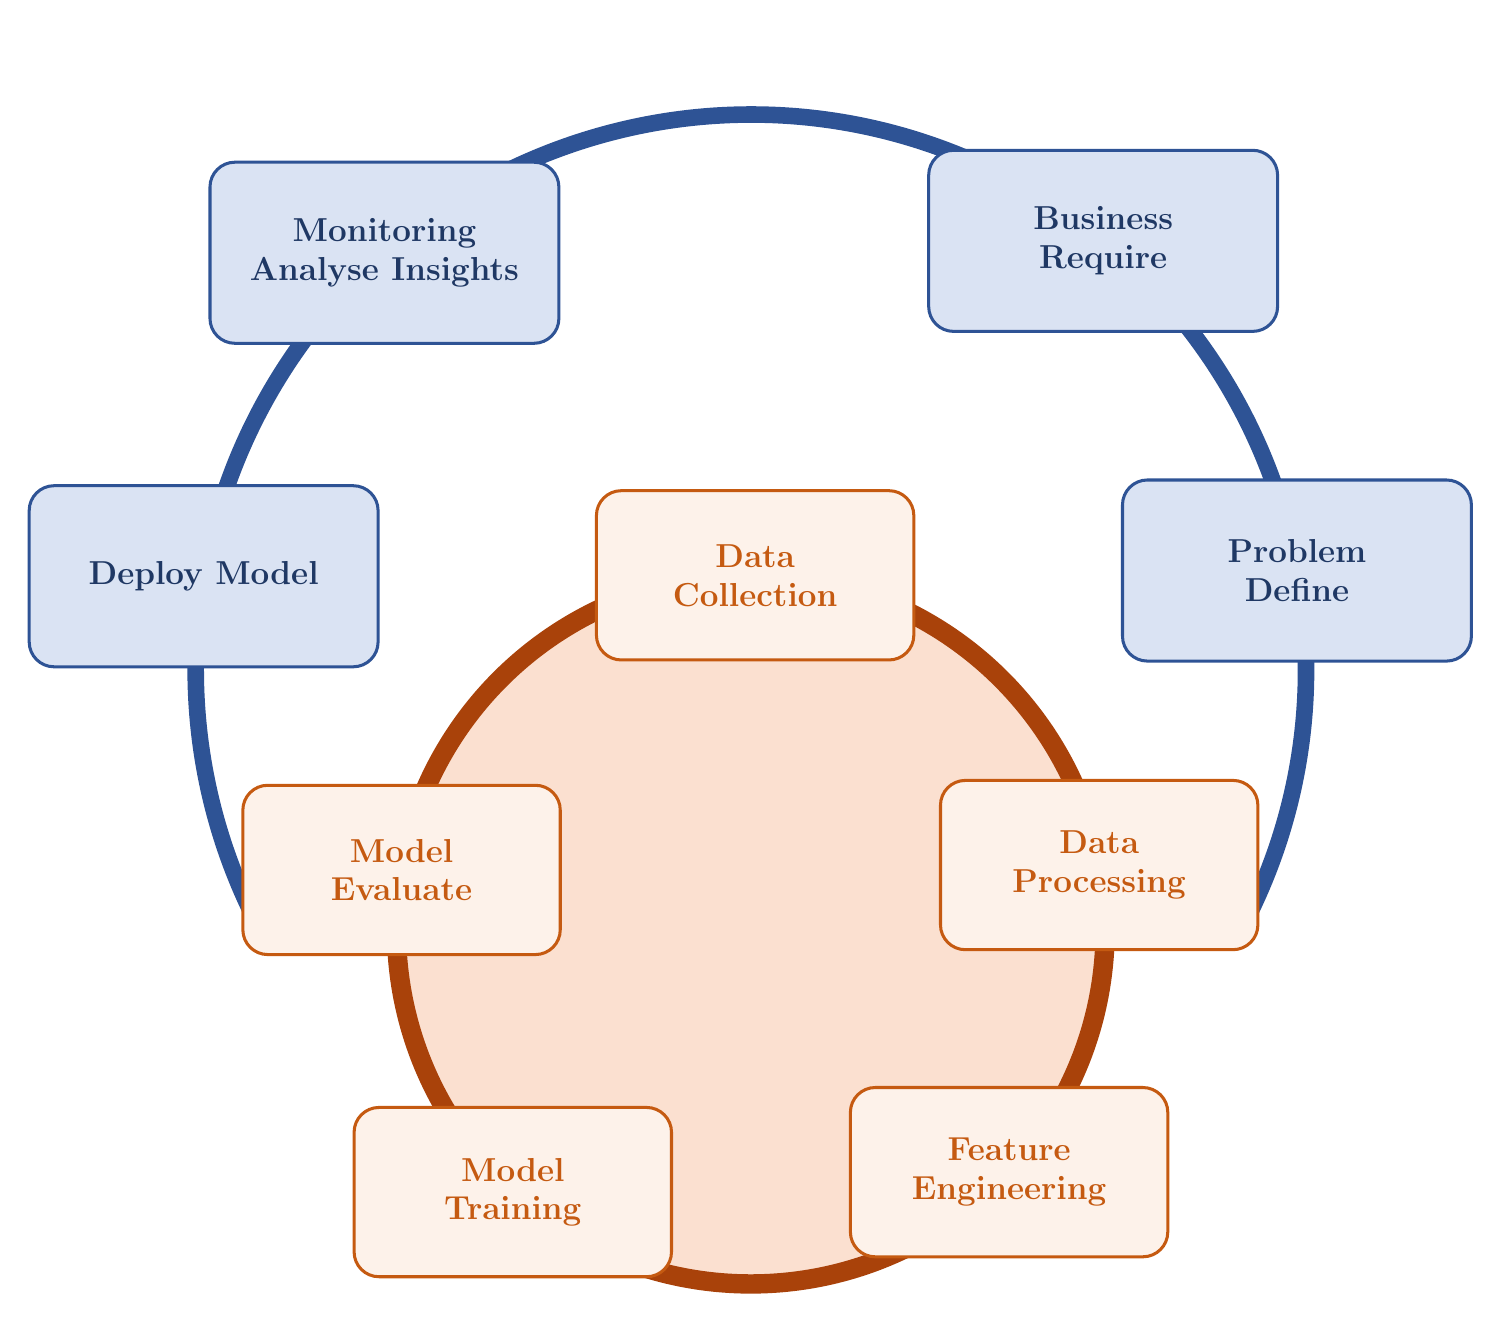
\begin{tikzpicture}[
  hopxanh/.style={
    draw=cXanhVien, line width=1.1pt, fill=cXanhNen, rounded corners=9pt,
    align=center, inner sep=4pt, text width=4.15cm, minimum height=2.3cm,
    font=\large\bfseries, text=cXanhChu
  },
  hopcam/.style={
    draw=cCamVien, line width=1.1pt, fill=cCamHop, rounded corners=9pt,
    align=center, inner sep=4pt, text width=3.75cm, minimum height=2.15cm,
    font=\large\bfseries, text=cCamVien
  }
]

% ── Hai duong tron: tam va ban kinh do tu ban goc ──
% Duong tron xanh : tam (0; 3,30) ban kinh 7,05 cm - chi ve cung tu -12 den 194 do
% Duong tron cam  : tam (0; 0)    ban kinh 4,50 cm - ve tron va to mau
\def\Rx{7.05}   \def\Cy{3.30}
\def\Rc{4.50}

% Dia tron cam ve TRUOC de cung xanh khong bi che
\fill[cCamNen] (0,0) circle (\Rc);
\draw[cCamVong, line width=7pt] (0,0) circle (\Rc);

% Cung tron xanh o ngoai. Hai dau keo den -27 va 207 do de diem cuoi nam HAN vao trong
% hop 'Xu ly du lieu' va 'Danh gia mo hinh'; hop ve sau nen che kin dau cung, nhin ra hai
% vong noi lien nhau dung nhu ban goc. De -12/194 do thi dau cung ho ra ngoai mep hop,
% thanh ra hai net xanh bi cut lung lo.
\draw[cXanhVien, line width=6pt]
  ([shift={(0,\Cy)}]-27:\Rx) arc[start angle=-27, end angle=207, radius=\Rx];

% ── Bon hop tren cung xanh ──
\node[hopxanh] at ($(0,\Cy)+(131.3:\Rx)$) {\Lmonitor};
\node[hopxanh] at ($(0,\Cy)+( 50.6:\Rx)$) {\Lbusiness};
\node[hopxanh] at ($(0,\Cy)+( 10.3:\Rx)$) {\Lproblem};
\node[hopxanh] at ($(0,\Cy)+(170.3:\Rx)$) {\Ldeploy};

% ── Nam hop tren vong cam ──
\node[hopcam] at ( 89.3:\Rc) {\Lcollect};
\node[hopcam] at ( 10.5:\Rc) {\Lprocess};
\node[hopcam] at (-43.2:\Rc) {\Lfeature};
\node[hopcam] at (227.8:\Rc) {\Ltrain};
\node[hopcam] at (170.3:\Rc) {\Levaluate};

\end{tikzpicture}
\end{document}
"
%    xelatex -jobname=sodo_ml_lifecycle_vi "\def\LANGVI{1}% =============================================================================
%  So do VONG DOI HOC MAY (ML Life Cycle) - ve lai tu slide 9 cua tai lieu
%  Data_Version_Control_V3.pdf (AI VIET NAM, All-in-One 2025).
%
%  Ve lai DUNG BO CUC goc: 1 cung tron mau xanh o ngoai mang 4 hop, 1 vong tron
%  to mau cam o trong mang 5 hop. Toa do goc do bang cach do lai vi tri tam va
%  ban kinh hai duong tron tren anh render 150 dpi cua slide, roi doi ra cm.
%
%  KHONG chep logo, tieu de slide, thanh mau va so trang cua tai lieu goc - do la
%  nhan dien thuong hieu cua ho, dua vao luan van se thanh mao nhan. Chi ve lai
%  phan so do.
%
%  Dung lai HAI ban:
%    xelatex -jobname=sodo_ml_lifecycle_en "\def\LANGVI{0}\input{sodo_ml_lifecycle_nguon.tex}"
%    xelatex -jobname=sodo_ml_lifecycle_vi "\def\LANGVI{1}\input{sodo_ml_lifecycle_nguon.tex}"
%
%  GHI CHU: ban goc viet sai chinh ta "Model Traing". Ban ve lai dung
%  "Model Training". Muon giu nguyen loi cua ban goc thi sua lai o \Ltrain.
% =============================================================================
\documentclass[12pt]{article}
\usepackage{fontspec}
\setmainfont{TeX Gyre Termes}          % chu co chan, khop kieu chu ban goc
% Khung giay do vua voi so do: TikZ do duoc 522,2 x 447,7 pt = 18,4 x 15,8 cm,
% cong dong tieu de va le nen cao 18,5 cm thi hinh nam gon 1 trang, khong bi day sang trang 2.
\usepackage[margin=0.5cm,paperwidth=19.5cm,paperheight=18.5cm]{geometry}
\usepackage{tikz}
\usetikzlibrary{arrows.meta,calc}
\pagestyle{empty}

% ── Bang mau lay tu anh render cua slide goc ──
\definecolor{cXanhVien}{HTML}{2E5395}   % vien va cung tron xanh
\definecolor{cXanhNen}{HTML}{DAE3F3}    % nen hop xanh
\definecolor{cXanhChu}{HTML}{1F3864}    % chu trong hop xanh
\definecolor{cCamVien}{HTML}{C55A11}    % vien hop cam va chu cam
\definecolor{cCamVong}{HTML}{A9420A}    % vanh tron cam dam
\definecolor{cCamNen}{HTML}{FBE0D0}     % nen dia tron cam
\definecolor{cCamHop}{HTML}{FDF2EA}     % nen hop cam

% ── Nhan hai ngon ngu ──
\providecommand{\LANGVI}{0}
\ifnum\LANGVI=1
  \def\Ltieude{Vòng đời học máy}
  \def\Lmonitor{Giám sát\\Phân tích thông tin}
  \def\Lbusiness{Yêu cầu\\nghiệp vụ}
  \def\Lproblem{Xác định\\bài toán}
  \def\Ldeploy{Triển khai mô hình}
  \def\Lcollect{Thu thập\\dữ liệu}
  \def\Lprocess{Xử lý\\dữ liệu}
  \def\Lfeature{Sinh\\đặc trưng}
  \def\Ltrain{Huấn luyện\\mô hình}
  \def\Levaluate{Đánh giá\\mô hình}
\else
  \def\Ltieude{ML Life Cycle}
  \def\Lmonitor{Monitoring\\Analyse Insights}
  \def\Lbusiness{Business\\Require}
  \def\Lproblem{Problem\\Define}
  \def\Ldeploy{Deploy Model}
  \def\Lcollect{Data\\Collection}
  \def\Lprocess{Data\\Processing}
  \def\Lfeature{Feature\\Engineering}
  \def\Ltrain{Model\\Training}
  \def\Levaluate{Model\\Evaluate}
\fi

\begin{document}
\noindent{\Large\bfseries\color{cXanhChu}$\diamond$~\Ltieude}\par
\vspace{2mm}
\centering
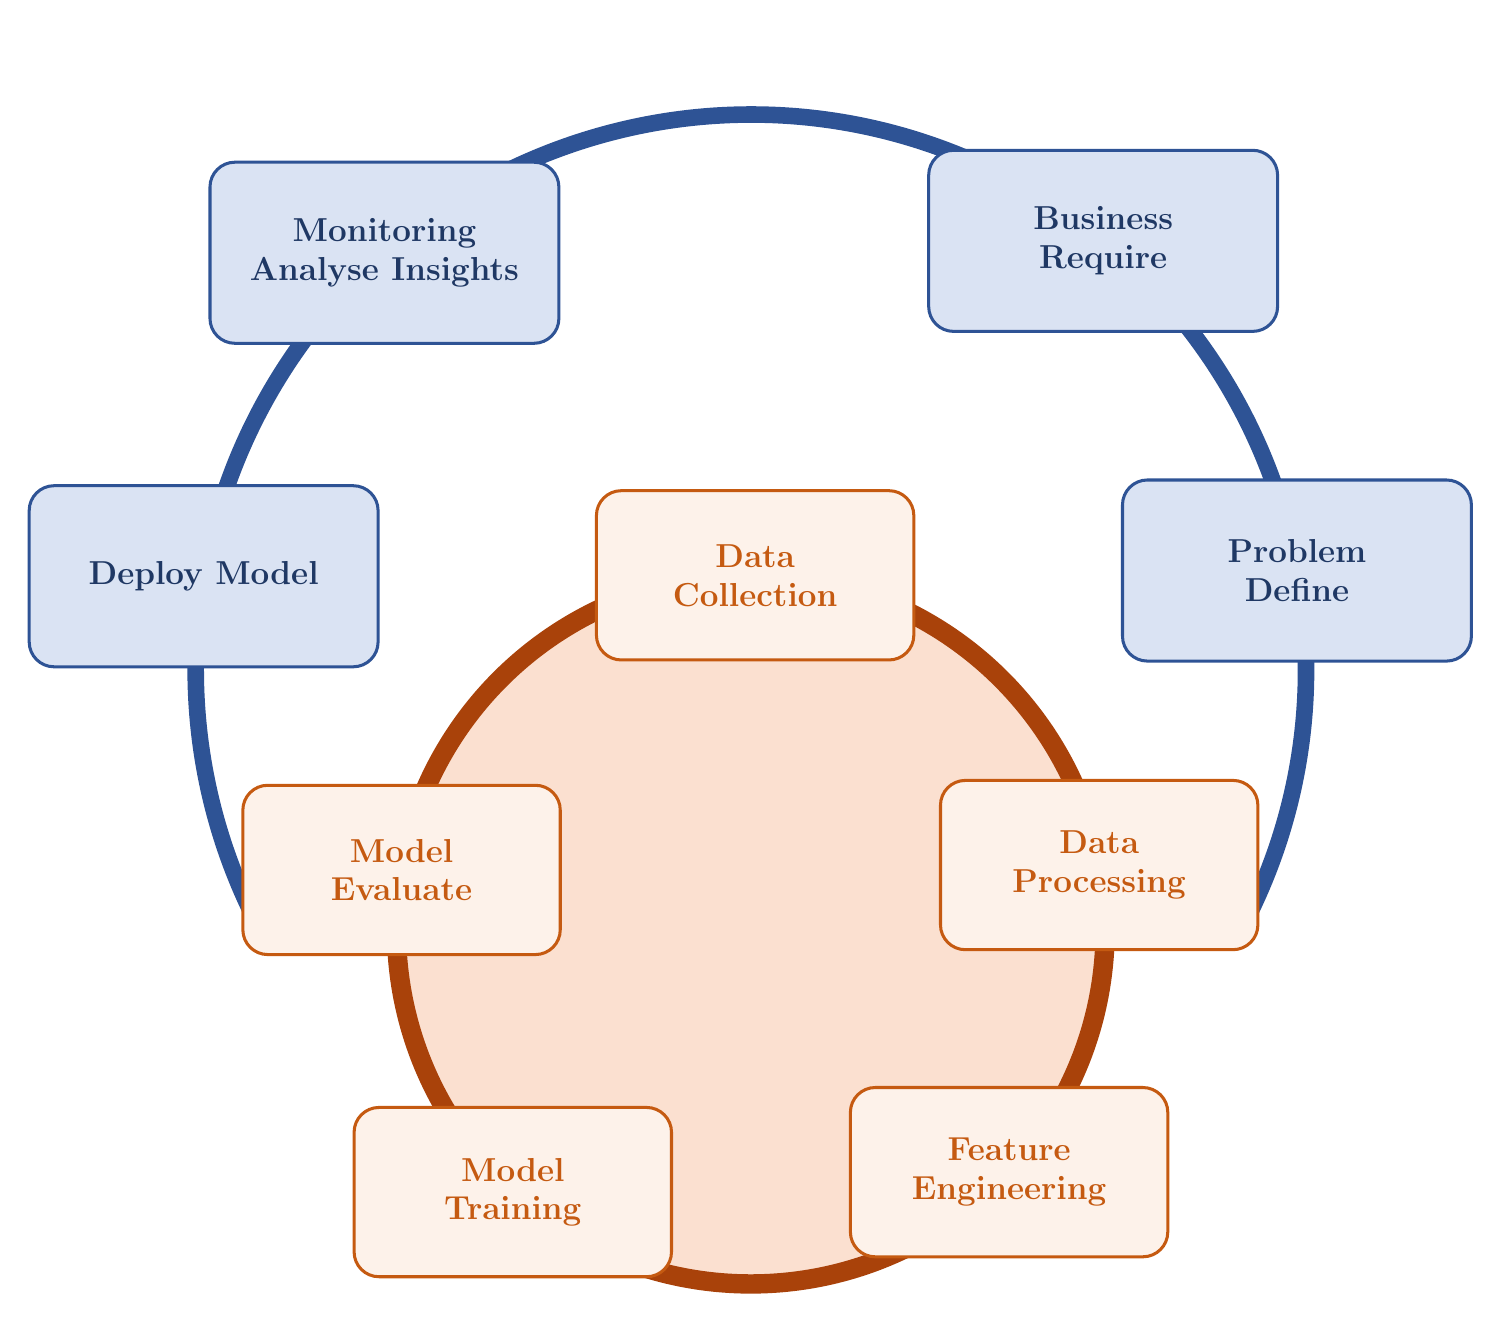
\begin{tikzpicture}[
  hopxanh/.style={
    draw=cXanhVien, line width=1.1pt, fill=cXanhNen, rounded corners=9pt,
    align=center, inner sep=4pt, text width=4.15cm, minimum height=2.3cm,
    font=\large\bfseries, text=cXanhChu
  },
  hopcam/.style={
    draw=cCamVien, line width=1.1pt, fill=cCamHop, rounded corners=9pt,
    align=center, inner sep=4pt, text width=3.75cm, minimum height=2.15cm,
    font=\large\bfseries, text=cCamVien
  }
]

% ── Hai duong tron: tam va ban kinh do tu ban goc ──
% Duong tron xanh : tam (0; 3,30) ban kinh 7,05 cm - chi ve cung tu -12 den 194 do
% Duong tron cam  : tam (0; 0)    ban kinh 4,50 cm - ve tron va to mau
\def\Rx{7.05}   \def\Cy{3.30}
\def\Rc{4.50}

% Dia tron cam ve TRUOC de cung xanh khong bi che
\fill[cCamNen] (0,0) circle (\Rc);
\draw[cCamVong, line width=7pt] (0,0) circle (\Rc);

% Cung tron xanh o ngoai. Hai dau keo den -27 va 207 do de diem cuoi nam HAN vao trong
% hop 'Xu ly du lieu' va 'Danh gia mo hinh'; hop ve sau nen che kin dau cung, nhin ra hai
% vong noi lien nhau dung nhu ban goc. De -12/194 do thi dau cung ho ra ngoai mep hop,
% thanh ra hai net xanh bi cut lung lo.
\draw[cXanhVien, line width=6pt]
  ([shift={(0,\Cy)}]-27:\Rx) arc[start angle=-27, end angle=207, radius=\Rx];

% ── Bon hop tren cung xanh ──
\node[hopxanh] at ($(0,\Cy)+(131.3:\Rx)$) {\Lmonitor};
\node[hopxanh] at ($(0,\Cy)+( 50.6:\Rx)$) {\Lbusiness};
\node[hopxanh] at ($(0,\Cy)+( 10.3:\Rx)$) {\Lproblem};
\node[hopxanh] at ($(0,\Cy)+(170.3:\Rx)$) {\Ldeploy};

% ── Nam hop tren vong cam ──
\node[hopcam] at ( 89.3:\Rc) {\Lcollect};
\node[hopcam] at ( 10.5:\Rc) {\Lprocess};
\node[hopcam] at (-43.2:\Rc) {\Lfeature};
\node[hopcam] at (227.8:\Rc) {\Ltrain};
\node[hopcam] at (170.3:\Rc) {\Levaluate};

\end{tikzpicture}
\end{document}
"
%
%  GHI CHU: ban goc viet sai chinh ta "Model Traing". Ban ve lai dung
%  "Model Training". Muon giu nguyen loi cua ban goc thi sua lai o \Ltrain.
% =============================================================================
\documentclass[12pt]{article}
\usepackage{fontspec}
\setmainfont{TeX Gyre Termes}          % chu co chan, khop kieu chu ban goc
% Khung giay do vua voi so do: TikZ do duoc 522,2 x 447,7 pt = 18,4 x 15,8 cm,
% cong dong tieu de va le nen cao 18,5 cm thi hinh nam gon 1 trang, khong bi day sang trang 2.
\usepackage[margin=0.5cm,paperwidth=19.5cm,paperheight=18.5cm]{geometry}
\usepackage{tikz}
\usetikzlibrary{arrows.meta,calc}
\pagestyle{empty}

% ── Bang mau lay tu anh render cua slide goc ──
\definecolor{cXanhVien}{HTML}{2E5395}   % vien va cung tron xanh
\definecolor{cXanhNen}{HTML}{DAE3F3}    % nen hop xanh
\definecolor{cXanhChu}{HTML}{1F3864}    % chu trong hop xanh
\definecolor{cCamVien}{HTML}{C55A11}    % vien hop cam va chu cam
\definecolor{cCamVong}{HTML}{A9420A}    % vanh tron cam dam
\definecolor{cCamNen}{HTML}{FBE0D0}     % nen dia tron cam
\definecolor{cCamHop}{HTML}{FDF2EA}     % nen hop cam

% ── Nhan hai ngon ngu ──
\providecommand{\LANGVI}{0}
\ifnum\LANGVI=1
  \def\Ltieude{Vòng đời học máy}
  \def\Lmonitor{Giám sát\\Phân tích thông tin}
  \def\Lbusiness{Yêu cầu\\nghiệp vụ}
  \def\Lproblem{Xác định\\bài toán}
  \def\Ldeploy{Triển khai mô hình}
  \def\Lcollect{Thu thập\\dữ liệu}
  \def\Lprocess{Xử lý\\dữ liệu}
  \def\Lfeature{Sinh\\đặc trưng}
  \def\Ltrain{Huấn luyện\\mô hình}
  \def\Levaluate{Đánh giá\\mô hình}
\else
  \def\Ltieude{ML Life Cycle}
  \def\Lmonitor{Monitoring\\Analyse Insights}
  \def\Lbusiness{Business\\Require}
  \def\Lproblem{Problem\\Define}
  \def\Ldeploy{Deploy Model}
  \def\Lcollect{Data\\Collection}
  \def\Lprocess{Data\\Processing}
  \def\Lfeature{Feature\\Engineering}
  \def\Ltrain{Model\\Training}
  \def\Levaluate{Model\\Evaluate}
\fi

\begin{document}
\noindent{\Large\bfseries\color{cXanhChu}$\diamond$~\Ltieude}\par
\vspace{2mm}
\centering
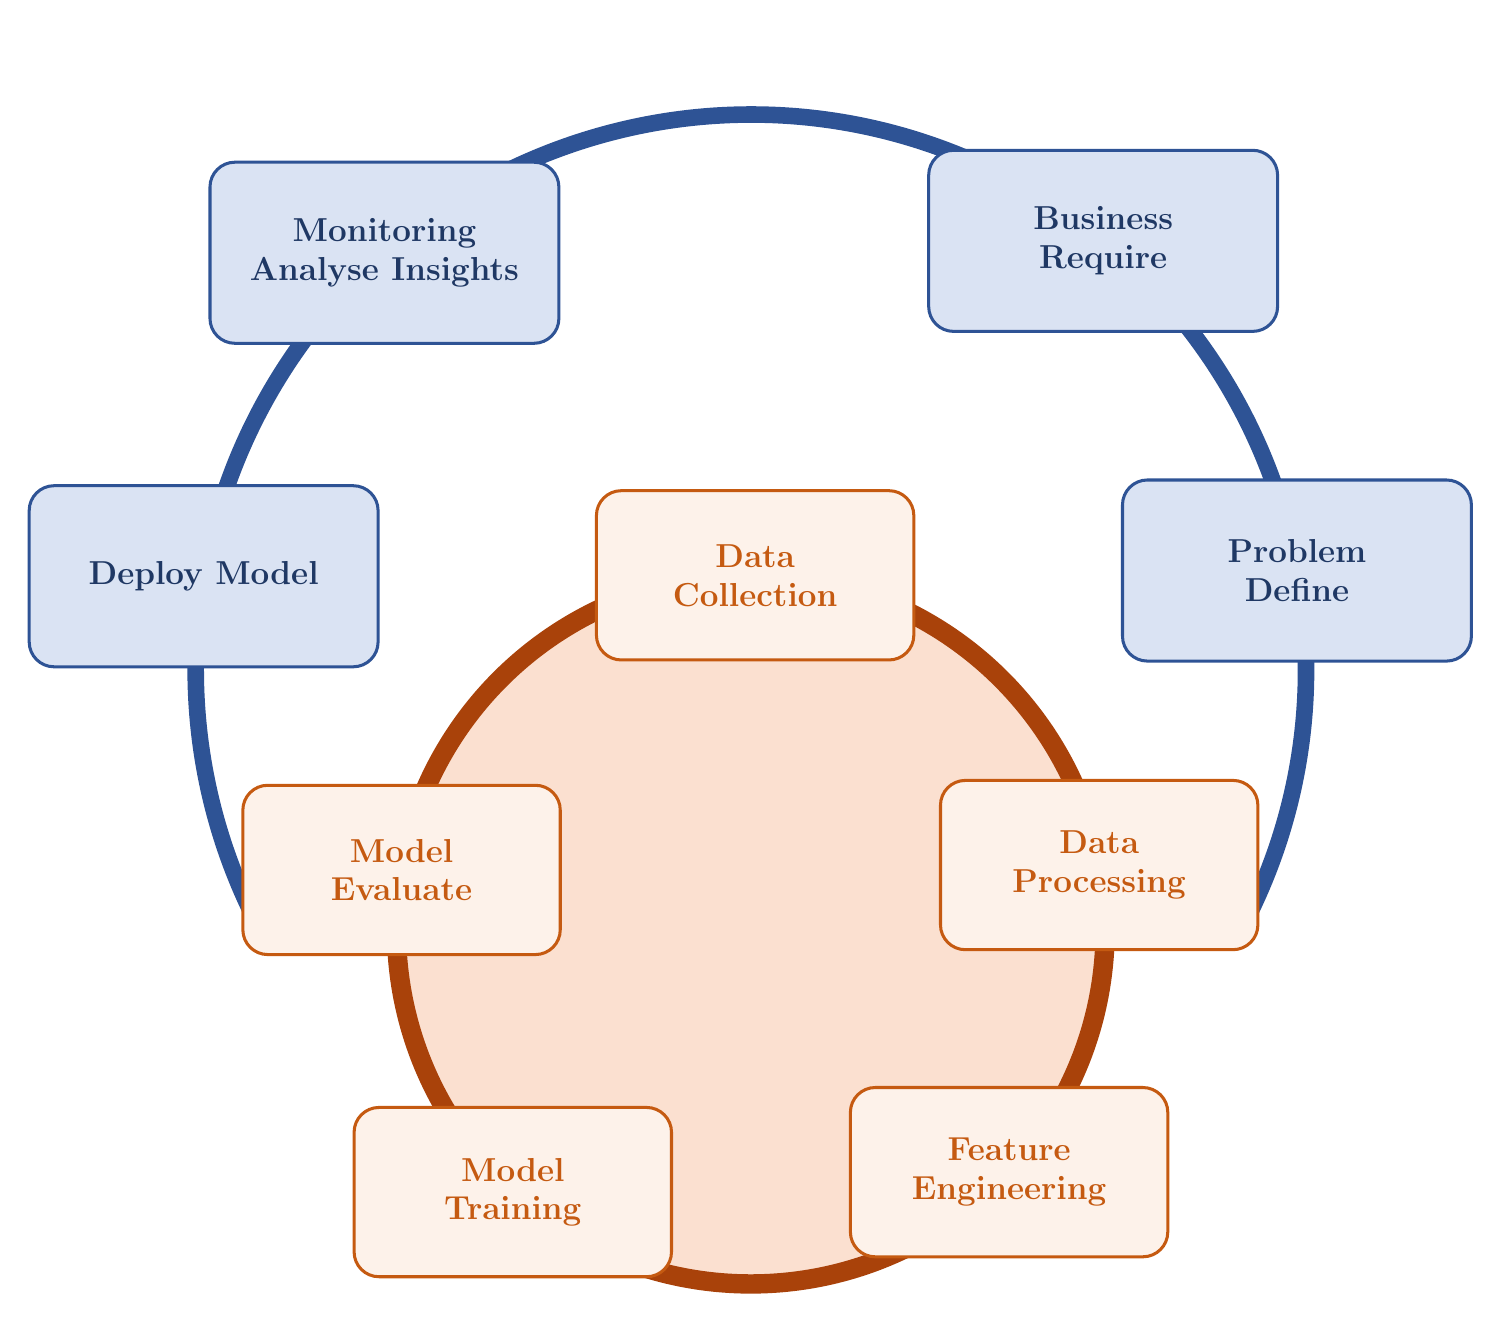
\begin{tikzpicture}[
  hopxanh/.style={
    draw=cXanhVien, line width=1.1pt, fill=cXanhNen, rounded corners=9pt,
    align=center, inner sep=4pt, text width=4.15cm, minimum height=2.3cm,
    font=\large\bfseries, text=cXanhChu
  },
  hopcam/.style={
    draw=cCamVien, line width=1.1pt, fill=cCamHop, rounded corners=9pt,
    align=center, inner sep=4pt, text width=3.75cm, minimum height=2.15cm,
    font=\large\bfseries, text=cCamVien
  }
]

% ── Hai duong tron: tam va ban kinh do tu ban goc ──
% Duong tron xanh : tam (0; 3,30) ban kinh 7,05 cm - chi ve cung tu -12 den 194 do
% Duong tron cam  : tam (0; 0)    ban kinh 4,50 cm - ve tron va to mau
\def\Rx{7.05}   \def\Cy{3.30}
\def\Rc{4.50}

% Dia tron cam ve TRUOC de cung xanh khong bi che
\fill[cCamNen] (0,0) circle (\Rc);
\draw[cCamVong, line width=7pt] (0,0) circle (\Rc);

% Cung tron xanh o ngoai. Hai dau keo den -27 va 207 do de diem cuoi nam HAN vao trong
% hop 'Xu ly du lieu' va 'Danh gia mo hinh'; hop ve sau nen che kin dau cung, nhin ra hai
% vong noi lien nhau dung nhu ban goc. De -12/194 do thi dau cung ho ra ngoai mep hop,
% thanh ra hai net xanh bi cut lung lo.
\draw[cXanhVien, line width=6pt]
  ([shift={(0,\Cy)}]-27:\Rx) arc[start angle=-27, end angle=207, radius=\Rx];

% ── Bon hop tren cung xanh ──
\node[hopxanh] at ($(0,\Cy)+(131.3:\Rx)$) {\Lmonitor};
\node[hopxanh] at ($(0,\Cy)+( 50.6:\Rx)$) {\Lbusiness};
\node[hopxanh] at ($(0,\Cy)+( 10.3:\Rx)$) {\Lproblem};
\node[hopxanh] at ($(0,\Cy)+(170.3:\Rx)$) {\Ldeploy};

% ── Nam hop tren vong cam ──
\node[hopcam] at ( 89.3:\Rc) {\Lcollect};
\node[hopcam] at ( 10.5:\Rc) {\Lprocess};
\node[hopcam] at (-43.2:\Rc) {\Lfeature};
\node[hopcam] at (227.8:\Rc) {\Ltrain};
\node[hopcam] at (170.3:\Rc) {\Levaluate};

\end{tikzpicture}
\end{document}
"
%    xelatex -jobname=sodo_ml_lifecycle_vi "\def\LANGVI{1}% =============================================================================
%  So do VONG DOI HOC MAY (ML Life Cycle) - ve lai tu slide 9 cua tai lieu
%  Data_Version_Control_V3.pdf (AI VIET NAM, All-in-One 2025).
%
%  Ve lai DUNG BO CUC goc: 1 cung tron mau xanh o ngoai mang 4 hop, 1 vong tron
%  to mau cam o trong mang 5 hop. Toa do goc do bang cach do lai vi tri tam va
%  ban kinh hai duong tron tren anh render 150 dpi cua slide, roi doi ra cm.
%
%  KHONG chep logo, tieu de slide, thanh mau va so trang cua tai lieu goc - do la
%  nhan dien thuong hieu cua ho, dua vao luan van se thanh mao nhan. Chi ve lai
%  phan so do.
%
%  Dung lai HAI ban:
%    xelatex -jobname=sodo_ml_lifecycle_en "\def\LANGVI{0}% =============================================================================
%  So do VONG DOI HOC MAY (ML Life Cycle) - ve lai tu slide 9 cua tai lieu
%  Data_Version_Control_V3.pdf (AI VIET NAM, All-in-One 2025).
%
%  Ve lai DUNG BO CUC goc: 1 cung tron mau xanh o ngoai mang 4 hop, 1 vong tron
%  to mau cam o trong mang 5 hop. Toa do goc do bang cach do lai vi tri tam va
%  ban kinh hai duong tron tren anh render 150 dpi cua slide, roi doi ra cm.
%
%  KHONG chep logo, tieu de slide, thanh mau va so trang cua tai lieu goc - do la
%  nhan dien thuong hieu cua ho, dua vao luan van se thanh mao nhan. Chi ve lai
%  phan so do.
%
%  Dung lai HAI ban:
%    xelatex -jobname=sodo_ml_lifecycle_en "\def\LANGVI{0}\input{sodo_ml_lifecycle_nguon.tex}"
%    xelatex -jobname=sodo_ml_lifecycle_vi "\def\LANGVI{1}\input{sodo_ml_lifecycle_nguon.tex}"
%
%  GHI CHU: ban goc viet sai chinh ta "Model Traing". Ban ve lai dung
%  "Model Training". Muon giu nguyen loi cua ban goc thi sua lai o \Ltrain.
% =============================================================================
\documentclass[12pt]{article}
\usepackage{fontspec}
\setmainfont{TeX Gyre Termes}          % chu co chan, khop kieu chu ban goc
% Khung giay do vua voi so do: TikZ do duoc 522,2 x 447,7 pt = 18,4 x 15,8 cm,
% cong dong tieu de va le nen cao 18,5 cm thi hinh nam gon 1 trang, khong bi day sang trang 2.
\usepackage[margin=0.5cm,paperwidth=19.5cm,paperheight=18.5cm]{geometry}
\usepackage{tikz}
\usetikzlibrary{arrows.meta,calc}
\pagestyle{empty}

% ── Bang mau lay tu anh render cua slide goc ──
\definecolor{cXanhVien}{HTML}{2E5395}   % vien va cung tron xanh
\definecolor{cXanhNen}{HTML}{DAE3F3}    % nen hop xanh
\definecolor{cXanhChu}{HTML}{1F3864}    % chu trong hop xanh
\definecolor{cCamVien}{HTML}{C55A11}    % vien hop cam va chu cam
\definecolor{cCamVong}{HTML}{A9420A}    % vanh tron cam dam
\definecolor{cCamNen}{HTML}{FBE0D0}     % nen dia tron cam
\definecolor{cCamHop}{HTML}{FDF2EA}     % nen hop cam

% ── Nhan hai ngon ngu ──
\providecommand{\LANGVI}{0}
\ifnum\LANGVI=1
  \def\Ltieude{Vòng đời học máy}
  \def\Lmonitor{Giám sát\\Phân tích thông tin}
  \def\Lbusiness{Yêu cầu\\nghiệp vụ}
  \def\Lproblem{Xác định\\bài toán}
  \def\Ldeploy{Triển khai mô hình}
  \def\Lcollect{Thu thập\\dữ liệu}
  \def\Lprocess{Xử lý\\dữ liệu}
  \def\Lfeature{Sinh\\đặc trưng}
  \def\Ltrain{Huấn luyện\\mô hình}
  \def\Levaluate{Đánh giá\\mô hình}
\else
  \def\Ltieude{ML Life Cycle}
  \def\Lmonitor{Monitoring\\Analyse Insights}
  \def\Lbusiness{Business\\Require}
  \def\Lproblem{Problem\\Define}
  \def\Ldeploy{Deploy Model}
  \def\Lcollect{Data\\Collection}
  \def\Lprocess{Data\\Processing}
  \def\Lfeature{Feature\\Engineering}
  \def\Ltrain{Model\\Training}
  \def\Levaluate{Model\\Evaluate}
\fi

\begin{document}
\noindent{\Large\bfseries\color{cXanhChu}$\diamond$~\Ltieude}\par
\vspace{2mm}
\centering
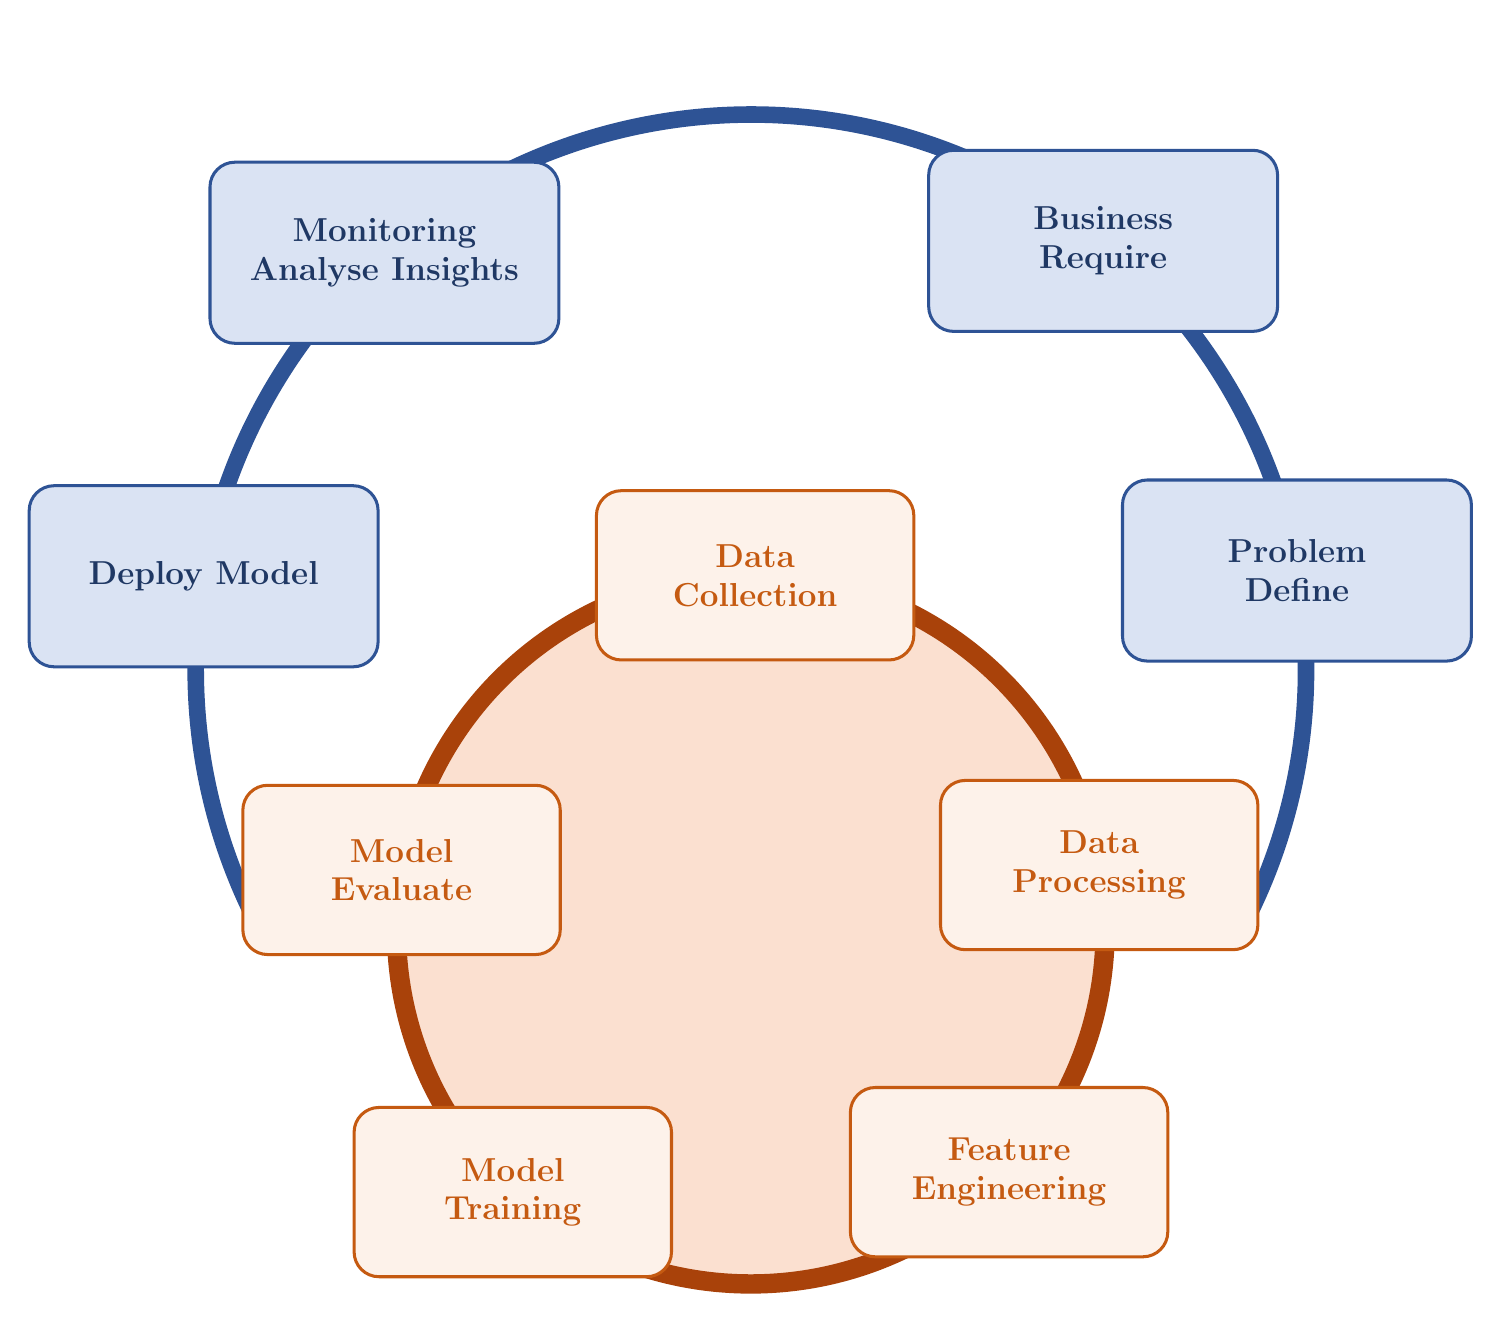
\begin{tikzpicture}[
  hopxanh/.style={
    draw=cXanhVien, line width=1.1pt, fill=cXanhNen, rounded corners=9pt,
    align=center, inner sep=4pt, text width=4.15cm, minimum height=2.3cm,
    font=\large\bfseries, text=cXanhChu
  },
  hopcam/.style={
    draw=cCamVien, line width=1.1pt, fill=cCamHop, rounded corners=9pt,
    align=center, inner sep=4pt, text width=3.75cm, minimum height=2.15cm,
    font=\large\bfseries, text=cCamVien
  }
]

% ── Hai duong tron: tam va ban kinh do tu ban goc ──
% Duong tron xanh : tam (0; 3,30) ban kinh 7,05 cm - chi ve cung tu -12 den 194 do
% Duong tron cam  : tam (0; 0)    ban kinh 4,50 cm - ve tron va to mau
\def\Rx{7.05}   \def\Cy{3.30}
\def\Rc{4.50}

% Dia tron cam ve TRUOC de cung xanh khong bi che
\fill[cCamNen] (0,0) circle (\Rc);
\draw[cCamVong, line width=7pt] (0,0) circle (\Rc);

% Cung tron xanh o ngoai. Hai dau keo den -27 va 207 do de diem cuoi nam HAN vao trong
% hop 'Xu ly du lieu' va 'Danh gia mo hinh'; hop ve sau nen che kin dau cung, nhin ra hai
% vong noi lien nhau dung nhu ban goc. De -12/194 do thi dau cung ho ra ngoai mep hop,
% thanh ra hai net xanh bi cut lung lo.
\draw[cXanhVien, line width=6pt]
  ([shift={(0,\Cy)}]-27:\Rx) arc[start angle=-27, end angle=207, radius=\Rx];

% ── Bon hop tren cung xanh ──
\node[hopxanh] at ($(0,\Cy)+(131.3:\Rx)$) {\Lmonitor};
\node[hopxanh] at ($(0,\Cy)+( 50.6:\Rx)$) {\Lbusiness};
\node[hopxanh] at ($(0,\Cy)+( 10.3:\Rx)$) {\Lproblem};
\node[hopxanh] at ($(0,\Cy)+(170.3:\Rx)$) {\Ldeploy};

% ── Nam hop tren vong cam ──
\node[hopcam] at ( 89.3:\Rc) {\Lcollect};
\node[hopcam] at ( 10.5:\Rc) {\Lprocess};
\node[hopcam] at (-43.2:\Rc) {\Lfeature};
\node[hopcam] at (227.8:\Rc) {\Ltrain};
\node[hopcam] at (170.3:\Rc) {\Levaluate};

\end{tikzpicture}
\end{document}
"
%    xelatex -jobname=sodo_ml_lifecycle_vi "\def\LANGVI{1}% =============================================================================
%  So do VONG DOI HOC MAY (ML Life Cycle) - ve lai tu slide 9 cua tai lieu
%  Data_Version_Control_V3.pdf (AI VIET NAM, All-in-One 2025).
%
%  Ve lai DUNG BO CUC goc: 1 cung tron mau xanh o ngoai mang 4 hop, 1 vong tron
%  to mau cam o trong mang 5 hop. Toa do goc do bang cach do lai vi tri tam va
%  ban kinh hai duong tron tren anh render 150 dpi cua slide, roi doi ra cm.
%
%  KHONG chep logo, tieu de slide, thanh mau va so trang cua tai lieu goc - do la
%  nhan dien thuong hieu cua ho, dua vao luan van se thanh mao nhan. Chi ve lai
%  phan so do.
%
%  Dung lai HAI ban:
%    xelatex -jobname=sodo_ml_lifecycle_en "\def\LANGVI{0}\input{sodo_ml_lifecycle_nguon.tex}"
%    xelatex -jobname=sodo_ml_lifecycle_vi "\def\LANGVI{1}\input{sodo_ml_lifecycle_nguon.tex}"
%
%  GHI CHU: ban goc viet sai chinh ta "Model Traing". Ban ve lai dung
%  "Model Training". Muon giu nguyen loi cua ban goc thi sua lai o \Ltrain.
% =============================================================================
\documentclass[12pt]{article}
\usepackage{fontspec}
\setmainfont{TeX Gyre Termes}          % chu co chan, khop kieu chu ban goc
% Khung giay do vua voi so do: TikZ do duoc 522,2 x 447,7 pt = 18,4 x 15,8 cm,
% cong dong tieu de va le nen cao 18,5 cm thi hinh nam gon 1 trang, khong bi day sang trang 2.
\usepackage[margin=0.5cm,paperwidth=19.5cm,paperheight=18.5cm]{geometry}
\usepackage{tikz}
\usetikzlibrary{arrows.meta,calc}
\pagestyle{empty}

% ── Bang mau lay tu anh render cua slide goc ──
\definecolor{cXanhVien}{HTML}{2E5395}   % vien va cung tron xanh
\definecolor{cXanhNen}{HTML}{DAE3F3}    % nen hop xanh
\definecolor{cXanhChu}{HTML}{1F3864}    % chu trong hop xanh
\definecolor{cCamVien}{HTML}{C55A11}    % vien hop cam va chu cam
\definecolor{cCamVong}{HTML}{A9420A}    % vanh tron cam dam
\definecolor{cCamNen}{HTML}{FBE0D0}     % nen dia tron cam
\definecolor{cCamHop}{HTML}{FDF2EA}     % nen hop cam

% ── Nhan hai ngon ngu ──
\providecommand{\LANGVI}{0}
\ifnum\LANGVI=1
  \def\Ltieude{Vòng đời học máy}
  \def\Lmonitor{Giám sát\\Phân tích thông tin}
  \def\Lbusiness{Yêu cầu\\nghiệp vụ}
  \def\Lproblem{Xác định\\bài toán}
  \def\Ldeploy{Triển khai mô hình}
  \def\Lcollect{Thu thập\\dữ liệu}
  \def\Lprocess{Xử lý\\dữ liệu}
  \def\Lfeature{Sinh\\đặc trưng}
  \def\Ltrain{Huấn luyện\\mô hình}
  \def\Levaluate{Đánh giá\\mô hình}
\else
  \def\Ltieude{ML Life Cycle}
  \def\Lmonitor{Monitoring\\Analyse Insights}
  \def\Lbusiness{Business\\Require}
  \def\Lproblem{Problem\\Define}
  \def\Ldeploy{Deploy Model}
  \def\Lcollect{Data\\Collection}
  \def\Lprocess{Data\\Processing}
  \def\Lfeature{Feature\\Engineering}
  \def\Ltrain{Model\\Training}
  \def\Levaluate{Model\\Evaluate}
\fi

\begin{document}
\noindent{\Large\bfseries\color{cXanhChu}$\diamond$~\Ltieude}\par
\vspace{2mm}
\centering
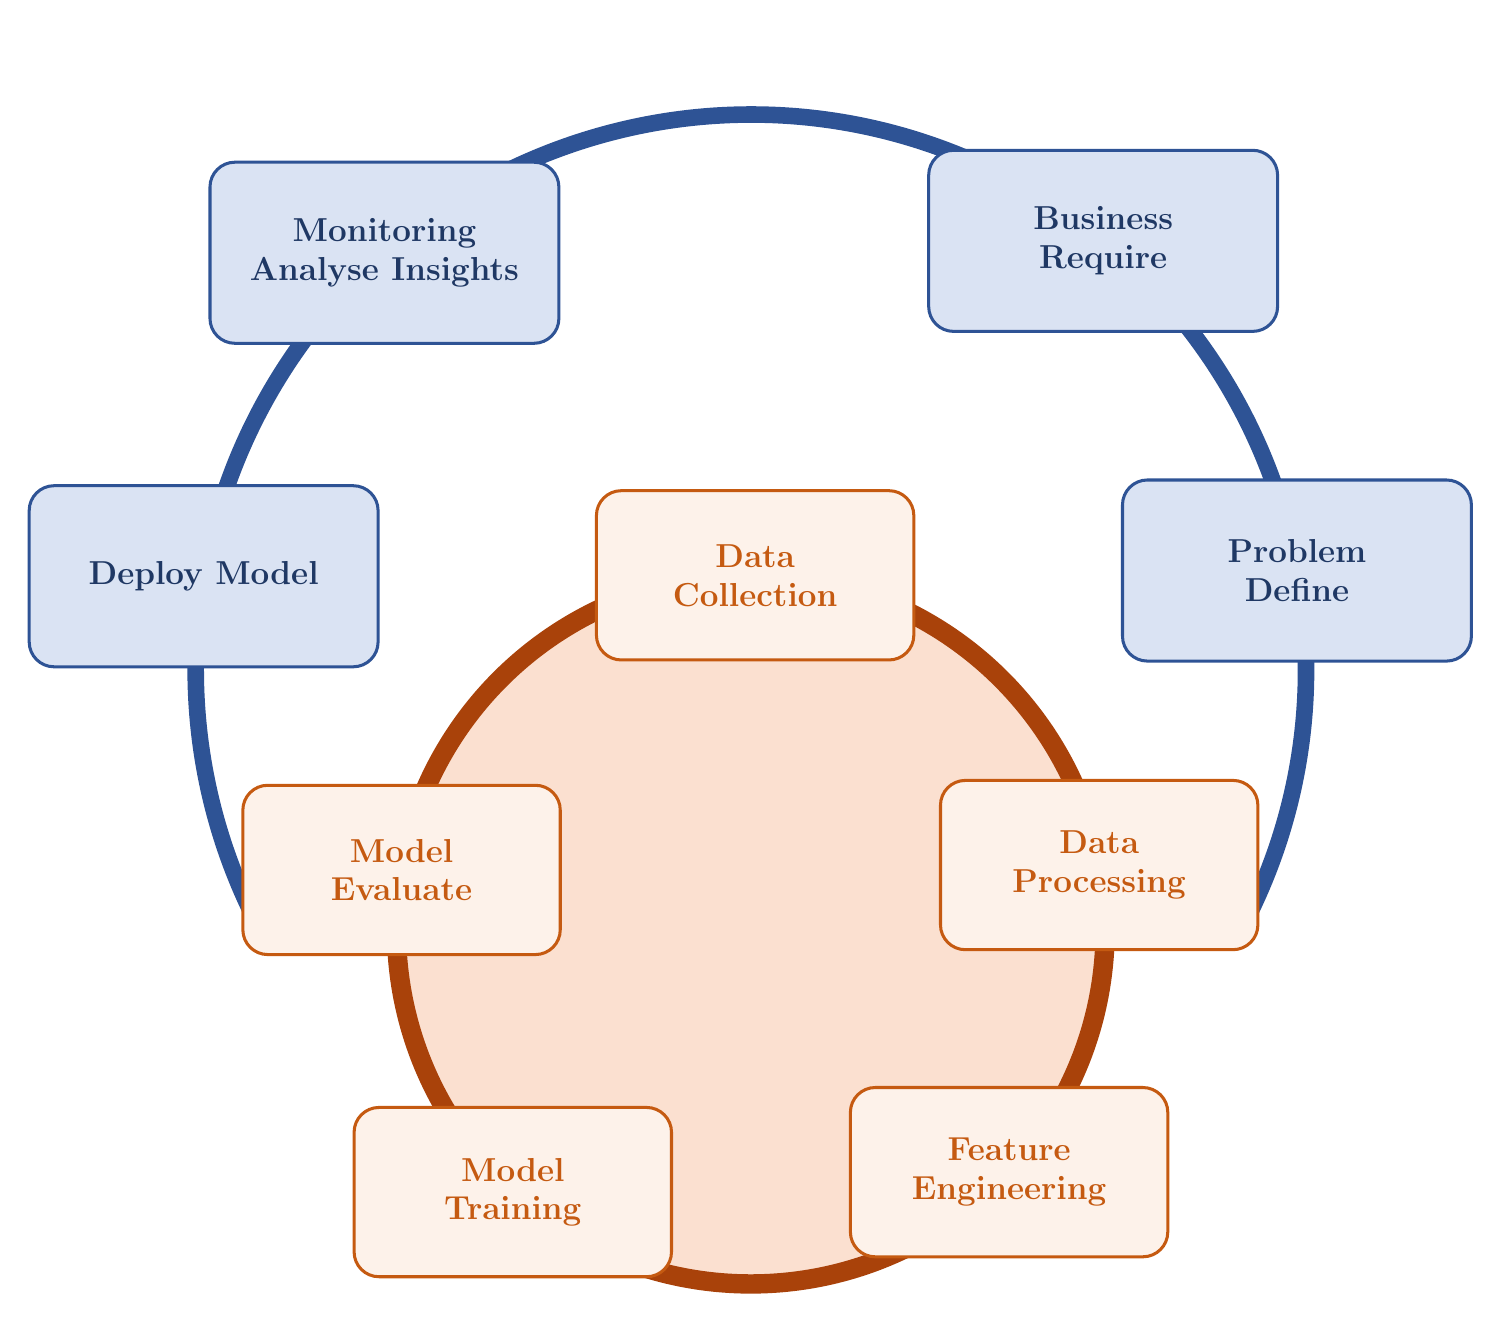
\begin{tikzpicture}[
  hopxanh/.style={
    draw=cXanhVien, line width=1.1pt, fill=cXanhNen, rounded corners=9pt,
    align=center, inner sep=4pt, text width=4.15cm, minimum height=2.3cm,
    font=\large\bfseries, text=cXanhChu
  },
  hopcam/.style={
    draw=cCamVien, line width=1.1pt, fill=cCamHop, rounded corners=9pt,
    align=center, inner sep=4pt, text width=3.75cm, minimum height=2.15cm,
    font=\large\bfseries, text=cCamVien
  }
]

% ── Hai duong tron: tam va ban kinh do tu ban goc ──
% Duong tron xanh : tam (0; 3,30) ban kinh 7,05 cm - chi ve cung tu -12 den 194 do
% Duong tron cam  : tam (0; 0)    ban kinh 4,50 cm - ve tron va to mau
\def\Rx{7.05}   \def\Cy{3.30}
\def\Rc{4.50}

% Dia tron cam ve TRUOC de cung xanh khong bi che
\fill[cCamNen] (0,0) circle (\Rc);
\draw[cCamVong, line width=7pt] (0,0) circle (\Rc);

% Cung tron xanh o ngoai. Hai dau keo den -27 va 207 do de diem cuoi nam HAN vao trong
% hop 'Xu ly du lieu' va 'Danh gia mo hinh'; hop ve sau nen che kin dau cung, nhin ra hai
% vong noi lien nhau dung nhu ban goc. De -12/194 do thi dau cung ho ra ngoai mep hop,
% thanh ra hai net xanh bi cut lung lo.
\draw[cXanhVien, line width=6pt]
  ([shift={(0,\Cy)}]-27:\Rx) arc[start angle=-27, end angle=207, radius=\Rx];

% ── Bon hop tren cung xanh ──
\node[hopxanh] at ($(0,\Cy)+(131.3:\Rx)$) {\Lmonitor};
\node[hopxanh] at ($(0,\Cy)+( 50.6:\Rx)$) {\Lbusiness};
\node[hopxanh] at ($(0,\Cy)+( 10.3:\Rx)$) {\Lproblem};
\node[hopxanh] at ($(0,\Cy)+(170.3:\Rx)$) {\Ldeploy};

% ── Nam hop tren vong cam ──
\node[hopcam] at ( 89.3:\Rc) {\Lcollect};
\node[hopcam] at ( 10.5:\Rc) {\Lprocess};
\node[hopcam] at (-43.2:\Rc) {\Lfeature};
\node[hopcam] at (227.8:\Rc) {\Ltrain};
\node[hopcam] at (170.3:\Rc) {\Levaluate};

\end{tikzpicture}
\end{document}
"
%
%  GHI CHU: ban goc viet sai chinh ta "Model Traing". Ban ve lai dung
%  "Model Training". Muon giu nguyen loi cua ban goc thi sua lai o \Ltrain.
% =============================================================================
\documentclass[12pt]{article}
\usepackage{fontspec}
\setmainfont{TeX Gyre Termes}          % chu co chan, khop kieu chu ban goc
% Khung giay do vua voi so do: TikZ do duoc 522,2 x 447,7 pt = 18,4 x 15,8 cm,
% cong dong tieu de va le nen cao 18,5 cm thi hinh nam gon 1 trang, khong bi day sang trang 2.
\usepackage[margin=0.5cm,paperwidth=19.5cm,paperheight=18.5cm]{geometry}
\usepackage{tikz}
\usetikzlibrary{arrows.meta,calc}
\pagestyle{empty}

% ── Bang mau lay tu anh render cua slide goc ──
\definecolor{cXanhVien}{HTML}{2E5395}   % vien va cung tron xanh
\definecolor{cXanhNen}{HTML}{DAE3F3}    % nen hop xanh
\definecolor{cXanhChu}{HTML}{1F3864}    % chu trong hop xanh
\definecolor{cCamVien}{HTML}{C55A11}    % vien hop cam va chu cam
\definecolor{cCamVong}{HTML}{A9420A}    % vanh tron cam dam
\definecolor{cCamNen}{HTML}{FBE0D0}     % nen dia tron cam
\definecolor{cCamHop}{HTML}{FDF2EA}     % nen hop cam

% ── Nhan hai ngon ngu ──
\providecommand{\LANGVI}{0}
\ifnum\LANGVI=1
  \def\Ltieude{Vòng đời học máy}
  \def\Lmonitor{Giám sát\\Phân tích thông tin}
  \def\Lbusiness{Yêu cầu\\nghiệp vụ}
  \def\Lproblem{Xác định\\bài toán}
  \def\Ldeploy{Triển khai mô hình}
  \def\Lcollect{Thu thập\\dữ liệu}
  \def\Lprocess{Xử lý\\dữ liệu}
  \def\Lfeature{Sinh\\đặc trưng}
  \def\Ltrain{Huấn luyện\\mô hình}
  \def\Levaluate{Đánh giá\\mô hình}
\else
  \def\Ltieude{ML Life Cycle}
  \def\Lmonitor{Monitoring\\Analyse Insights}
  \def\Lbusiness{Business\\Require}
  \def\Lproblem{Problem\\Define}
  \def\Ldeploy{Deploy Model}
  \def\Lcollect{Data\\Collection}
  \def\Lprocess{Data\\Processing}
  \def\Lfeature{Feature\\Engineering}
  \def\Ltrain{Model\\Training}
  \def\Levaluate{Model\\Evaluate}
\fi

\begin{document}
\noindent{\Large\bfseries\color{cXanhChu}$\diamond$~\Ltieude}\par
\vspace{2mm}
\centering
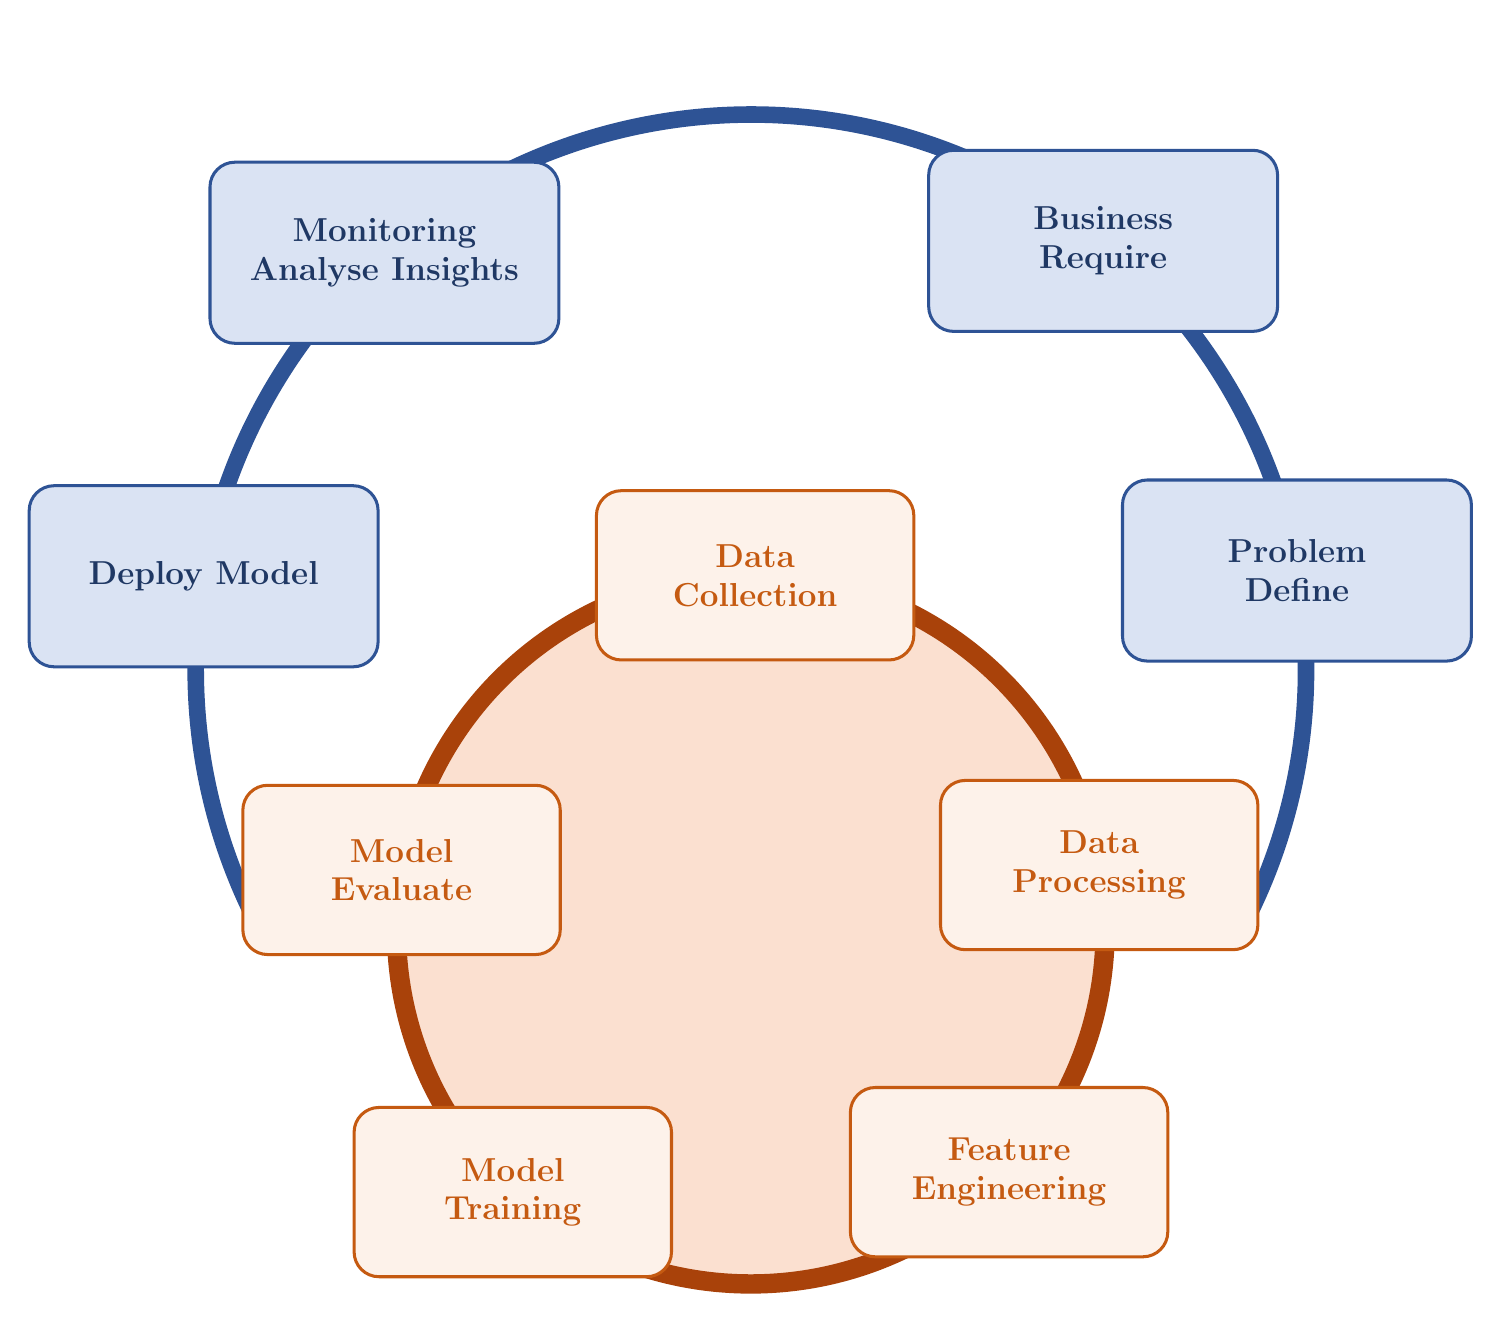
\begin{tikzpicture}[
  hopxanh/.style={
    draw=cXanhVien, line width=1.1pt, fill=cXanhNen, rounded corners=9pt,
    align=center, inner sep=4pt, text width=4.15cm, minimum height=2.3cm,
    font=\large\bfseries, text=cXanhChu
  },
  hopcam/.style={
    draw=cCamVien, line width=1.1pt, fill=cCamHop, rounded corners=9pt,
    align=center, inner sep=4pt, text width=3.75cm, minimum height=2.15cm,
    font=\large\bfseries, text=cCamVien
  }
]

% ── Hai duong tron: tam va ban kinh do tu ban goc ──
% Duong tron xanh : tam (0; 3,30) ban kinh 7,05 cm - chi ve cung tu -12 den 194 do
% Duong tron cam  : tam (0; 0)    ban kinh 4,50 cm - ve tron va to mau
\def\Rx{7.05}   \def\Cy{3.30}
\def\Rc{4.50}

% Dia tron cam ve TRUOC de cung xanh khong bi che
\fill[cCamNen] (0,0) circle (\Rc);
\draw[cCamVong, line width=7pt] (0,0) circle (\Rc);

% Cung tron xanh o ngoai. Hai dau keo den -27 va 207 do de diem cuoi nam HAN vao trong
% hop 'Xu ly du lieu' va 'Danh gia mo hinh'; hop ve sau nen che kin dau cung, nhin ra hai
% vong noi lien nhau dung nhu ban goc. De -12/194 do thi dau cung ho ra ngoai mep hop,
% thanh ra hai net xanh bi cut lung lo.
\draw[cXanhVien, line width=6pt]
  ([shift={(0,\Cy)}]-27:\Rx) arc[start angle=-27, end angle=207, radius=\Rx];

% ── Bon hop tren cung xanh ──
\node[hopxanh] at ($(0,\Cy)+(131.3:\Rx)$) {\Lmonitor};
\node[hopxanh] at ($(0,\Cy)+( 50.6:\Rx)$) {\Lbusiness};
\node[hopxanh] at ($(0,\Cy)+( 10.3:\Rx)$) {\Lproblem};
\node[hopxanh] at ($(0,\Cy)+(170.3:\Rx)$) {\Ldeploy};

% ── Nam hop tren vong cam ──
\node[hopcam] at ( 89.3:\Rc) {\Lcollect};
\node[hopcam] at ( 10.5:\Rc) {\Lprocess};
\node[hopcam] at (-43.2:\Rc) {\Lfeature};
\node[hopcam] at (227.8:\Rc) {\Ltrain};
\node[hopcam] at (170.3:\Rc) {\Levaluate};

\end{tikzpicture}
\end{document}
"
%
%  GHI CHU: ban goc viet sai chinh ta "Model Traing". Ban ve lai dung
%  "Model Training". Muon giu nguyen loi cua ban goc thi sua lai o \Ltrain.
% =============================================================================
\documentclass[12pt]{article}
\usepackage{fontspec}
\setmainfont{TeX Gyre Termes}          % chu co chan, khop kieu chu ban goc
% Khung giay do vua voi so do: TikZ do duoc 522,2 x 447,7 pt = 18,4 x 15,8 cm,
% cong dong tieu de va le nen cao 18,5 cm thi hinh nam gon 1 trang, khong bi day sang trang 2.
\usepackage[margin=0.5cm,paperwidth=19.5cm,paperheight=18.5cm]{geometry}
\usepackage{tikz}
\usetikzlibrary{arrows.meta,calc}
\pagestyle{empty}

% ── Bang mau lay tu anh render cua slide goc ──
\definecolor{cXanhVien}{HTML}{2E5395}   % vien va cung tron xanh
\definecolor{cXanhNen}{HTML}{DAE3F3}    % nen hop xanh
\definecolor{cXanhChu}{HTML}{1F3864}    % chu trong hop xanh
\definecolor{cCamVien}{HTML}{C55A11}    % vien hop cam va chu cam
\definecolor{cCamVong}{HTML}{A9420A}    % vanh tron cam dam
\definecolor{cCamNen}{HTML}{FBE0D0}     % nen dia tron cam
\definecolor{cCamHop}{HTML}{FDF2EA}     % nen hop cam

% ── Nhan hai ngon ngu ──
\providecommand{\LANGVI}{0}
\ifnum\LANGVI=1
  \def\Ltieude{Vòng đời học máy}
  \def\Lmonitor{Giám sát\\Phân tích thông tin}
  \def\Lbusiness{Yêu cầu\\nghiệp vụ}
  \def\Lproblem{Xác định\\bài toán}
  \def\Ldeploy{Triển khai mô hình}
  \def\Lcollect{Thu thập\\dữ liệu}
  \def\Lprocess{Xử lý\\dữ liệu}
  \def\Lfeature{Sinh\\đặc trưng}
  \def\Ltrain{Huấn luyện\\mô hình}
  \def\Levaluate{Đánh giá\\mô hình}
\else
  \def\Ltieude{ML Life Cycle}
  \def\Lmonitor{Monitoring\\Analyse Insights}
  \def\Lbusiness{Business\\Require}
  \def\Lproblem{Problem\\Define}
  \def\Ldeploy{Deploy Model}
  \def\Lcollect{Data\\Collection}
  \def\Lprocess{Data\\Processing}
  \def\Lfeature{Feature\\Engineering}
  \def\Ltrain{Model\\Training}
  \def\Levaluate{Model\\Evaluate}
\fi

\begin{document}
\noindent{\Large\bfseries\color{cXanhChu}$\diamond$~\Ltieude}\par
\vspace{2mm}
\centering
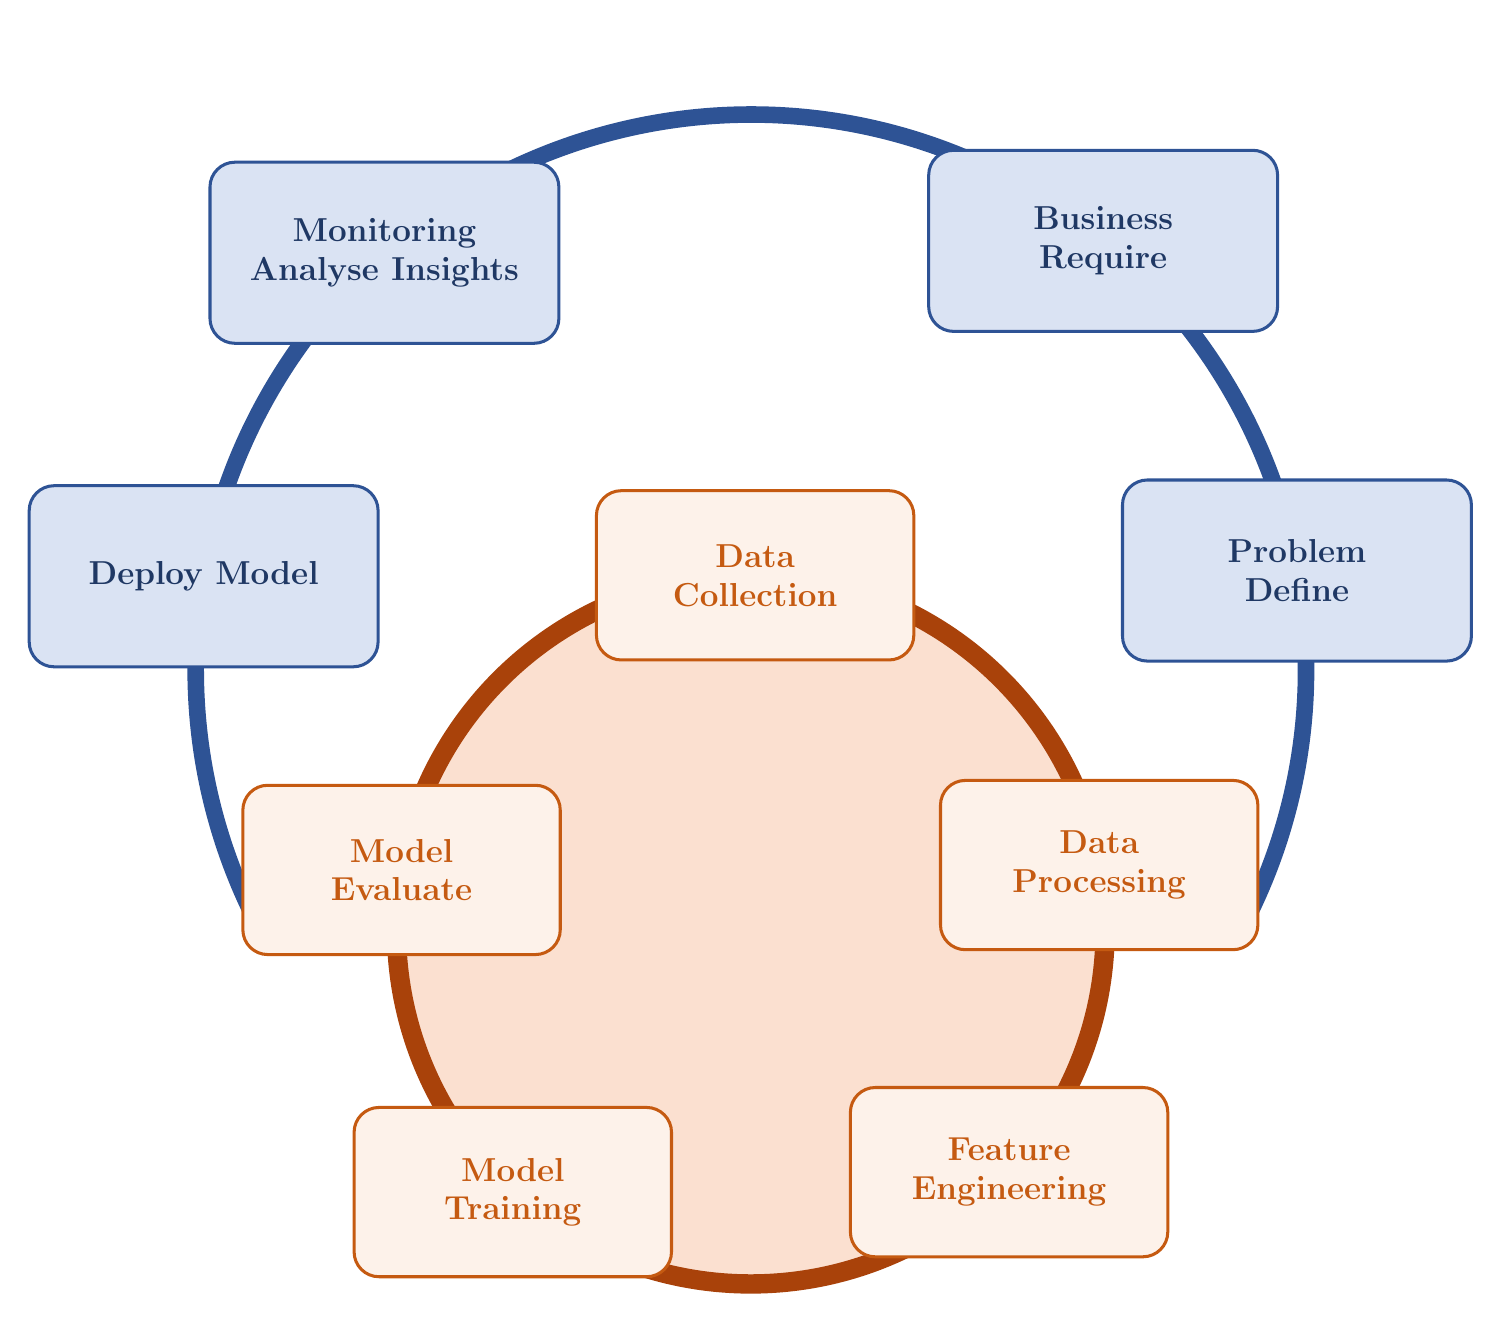
\begin{tikzpicture}[
  hopxanh/.style={
    draw=cXanhVien, line width=1.1pt, fill=cXanhNen, rounded corners=9pt,
    align=center, inner sep=4pt, text width=4.15cm, minimum height=2.3cm,
    font=\large\bfseries, text=cXanhChu
  },
  hopcam/.style={
    draw=cCamVien, line width=1.1pt, fill=cCamHop, rounded corners=9pt,
    align=center, inner sep=4pt, text width=3.75cm, minimum height=2.15cm,
    font=\large\bfseries, text=cCamVien
  }
]

% ── Hai duong tron: tam va ban kinh do tu ban goc ──
% Duong tron xanh : tam (0; 3,30) ban kinh 7,05 cm - chi ve cung tu -12 den 194 do
% Duong tron cam  : tam (0; 0)    ban kinh 4,50 cm - ve tron va to mau
\def\Rx{7.05}   \def\Cy{3.30}
\def\Rc{4.50}

% Dia tron cam ve TRUOC de cung xanh khong bi che
\fill[cCamNen] (0,0) circle (\Rc);
\draw[cCamVong, line width=7pt] (0,0) circle (\Rc);

% Cung tron xanh o ngoai. Hai dau keo den -27 va 207 do de diem cuoi nam HAN vao trong
% hop 'Xu ly du lieu' va 'Danh gia mo hinh'; hop ve sau nen che kin dau cung, nhin ra hai
% vong noi lien nhau dung nhu ban goc. De -12/194 do thi dau cung ho ra ngoai mep hop,
% thanh ra hai net xanh bi cut lung lo.
\draw[cXanhVien, line width=6pt]
  ([shift={(0,\Cy)}]-27:\Rx) arc[start angle=-27, end angle=207, radius=\Rx];

% ── Bon hop tren cung xanh ──
\node[hopxanh] at ($(0,\Cy)+(131.3:\Rx)$) {\Lmonitor};
\node[hopxanh] at ($(0,\Cy)+( 50.6:\Rx)$) {\Lbusiness};
\node[hopxanh] at ($(0,\Cy)+( 10.3:\Rx)$) {\Lproblem};
\node[hopxanh] at ($(0,\Cy)+(170.3:\Rx)$) {\Ldeploy};

% ── Nam hop tren vong cam ──
\node[hopcam] at ( 89.3:\Rc) {\Lcollect};
\node[hopcam] at ( 10.5:\Rc) {\Lprocess};
\node[hopcam] at (-43.2:\Rc) {\Lfeature};
\node[hopcam] at (227.8:\Rc) {\Ltrain};
\node[hopcam] at (170.3:\Rc) {\Levaluate};

\end{tikzpicture}
\end{document}
"
%    xelatex -jobname=sodo_ml_lifecycle_vi "\def\LANGVI{1}% =============================================================================
%  So do VONG DOI HOC MAY (ML Life Cycle) - ve lai tu slide 9 cua tai lieu
%  Data_Version_Control_V3.pdf (AI VIET NAM, All-in-One 2025).
%
%  Ve lai DUNG BO CUC goc: 1 cung tron mau xanh o ngoai mang 4 hop, 1 vong tron
%  to mau cam o trong mang 5 hop. Toa do goc do bang cach do lai vi tri tam va
%  ban kinh hai duong tron tren anh render 150 dpi cua slide, roi doi ra cm.
%
%  KHONG chep logo, tieu de slide, thanh mau va so trang cua tai lieu goc - do la
%  nhan dien thuong hieu cua ho, dua vao luan van se thanh mao nhan. Chi ve lai
%  phan so do.
%
%  Dung lai HAI ban:
%    xelatex -jobname=sodo_ml_lifecycle_en "\def\LANGVI{0}% =============================================================================
%  So do VONG DOI HOC MAY (ML Life Cycle) - ve lai tu slide 9 cua tai lieu
%  Data_Version_Control_V3.pdf (AI VIET NAM, All-in-One 2025).
%
%  Ve lai DUNG BO CUC goc: 1 cung tron mau xanh o ngoai mang 4 hop, 1 vong tron
%  to mau cam o trong mang 5 hop. Toa do goc do bang cach do lai vi tri tam va
%  ban kinh hai duong tron tren anh render 150 dpi cua slide, roi doi ra cm.
%
%  KHONG chep logo, tieu de slide, thanh mau va so trang cua tai lieu goc - do la
%  nhan dien thuong hieu cua ho, dua vao luan van se thanh mao nhan. Chi ve lai
%  phan so do.
%
%  Dung lai HAI ban:
%    xelatex -jobname=sodo_ml_lifecycle_en "\def\LANGVI{0}% =============================================================================
%  So do VONG DOI HOC MAY (ML Life Cycle) - ve lai tu slide 9 cua tai lieu
%  Data_Version_Control_V3.pdf (AI VIET NAM, All-in-One 2025).
%
%  Ve lai DUNG BO CUC goc: 1 cung tron mau xanh o ngoai mang 4 hop, 1 vong tron
%  to mau cam o trong mang 5 hop. Toa do goc do bang cach do lai vi tri tam va
%  ban kinh hai duong tron tren anh render 150 dpi cua slide, roi doi ra cm.
%
%  KHONG chep logo, tieu de slide, thanh mau va so trang cua tai lieu goc - do la
%  nhan dien thuong hieu cua ho, dua vao luan van se thanh mao nhan. Chi ve lai
%  phan so do.
%
%  Dung lai HAI ban:
%    xelatex -jobname=sodo_ml_lifecycle_en "\def\LANGVI{0}\input{sodo_ml_lifecycle_nguon.tex}"
%    xelatex -jobname=sodo_ml_lifecycle_vi "\def\LANGVI{1}\input{sodo_ml_lifecycle_nguon.tex}"
%
%  GHI CHU: ban goc viet sai chinh ta "Model Traing". Ban ve lai dung
%  "Model Training". Muon giu nguyen loi cua ban goc thi sua lai o \Ltrain.
% =============================================================================
\documentclass[12pt]{article}
\usepackage{fontspec}
\setmainfont{TeX Gyre Termes}          % chu co chan, khop kieu chu ban goc
% Khung giay do vua voi so do: TikZ do duoc 522,2 x 447,7 pt = 18,4 x 15,8 cm,
% cong dong tieu de va le nen cao 18,5 cm thi hinh nam gon 1 trang, khong bi day sang trang 2.
\usepackage[margin=0.5cm,paperwidth=19.5cm,paperheight=18.5cm]{geometry}
\usepackage{tikz}
\usetikzlibrary{arrows.meta,calc}
\pagestyle{empty}

% ── Bang mau lay tu anh render cua slide goc ──
\definecolor{cXanhVien}{HTML}{2E5395}   % vien va cung tron xanh
\definecolor{cXanhNen}{HTML}{DAE3F3}    % nen hop xanh
\definecolor{cXanhChu}{HTML}{1F3864}    % chu trong hop xanh
\definecolor{cCamVien}{HTML}{C55A11}    % vien hop cam va chu cam
\definecolor{cCamVong}{HTML}{A9420A}    % vanh tron cam dam
\definecolor{cCamNen}{HTML}{FBE0D0}     % nen dia tron cam
\definecolor{cCamHop}{HTML}{FDF2EA}     % nen hop cam

% ── Nhan hai ngon ngu ──
\providecommand{\LANGVI}{0}
\ifnum\LANGVI=1
  \def\Ltieude{Vòng đời học máy}
  \def\Lmonitor{Giám sát\\Phân tích thông tin}
  \def\Lbusiness{Yêu cầu\\nghiệp vụ}
  \def\Lproblem{Xác định\\bài toán}
  \def\Ldeploy{Triển khai mô hình}
  \def\Lcollect{Thu thập\\dữ liệu}
  \def\Lprocess{Xử lý\\dữ liệu}
  \def\Lfeature{Sinh\\đặc trưng}
  \def\Ltrain{Huấn luyện\\mô hình}
  \def\Levaluate{Đánh giá\\mô hình}
\else
  \def\Ltieude{ML Life Cycle}
  \def\Lmonitor{Monitoring\\Analyse Insights}
  \def\Lbusiness{Business\\Require}
  \def\Lproblem{Problem\\Define}
  \def\Ldeploy{Deploy Model}
  \def\Lcollect{Data\\Collection}
  \def\Lprocess{Data\\Processing}
  \def\Lfeature{Feature\\Engineering}
  \def\Ltrain{Model\\Training}
  \def\Levaluate{Model\\Evaluate}
\fi

\begin{document}
\noindent{\Large\bfseries\color{cXanhChu}$\diamond$~\Ltieude}\par
\vspace{2mm}
\centering
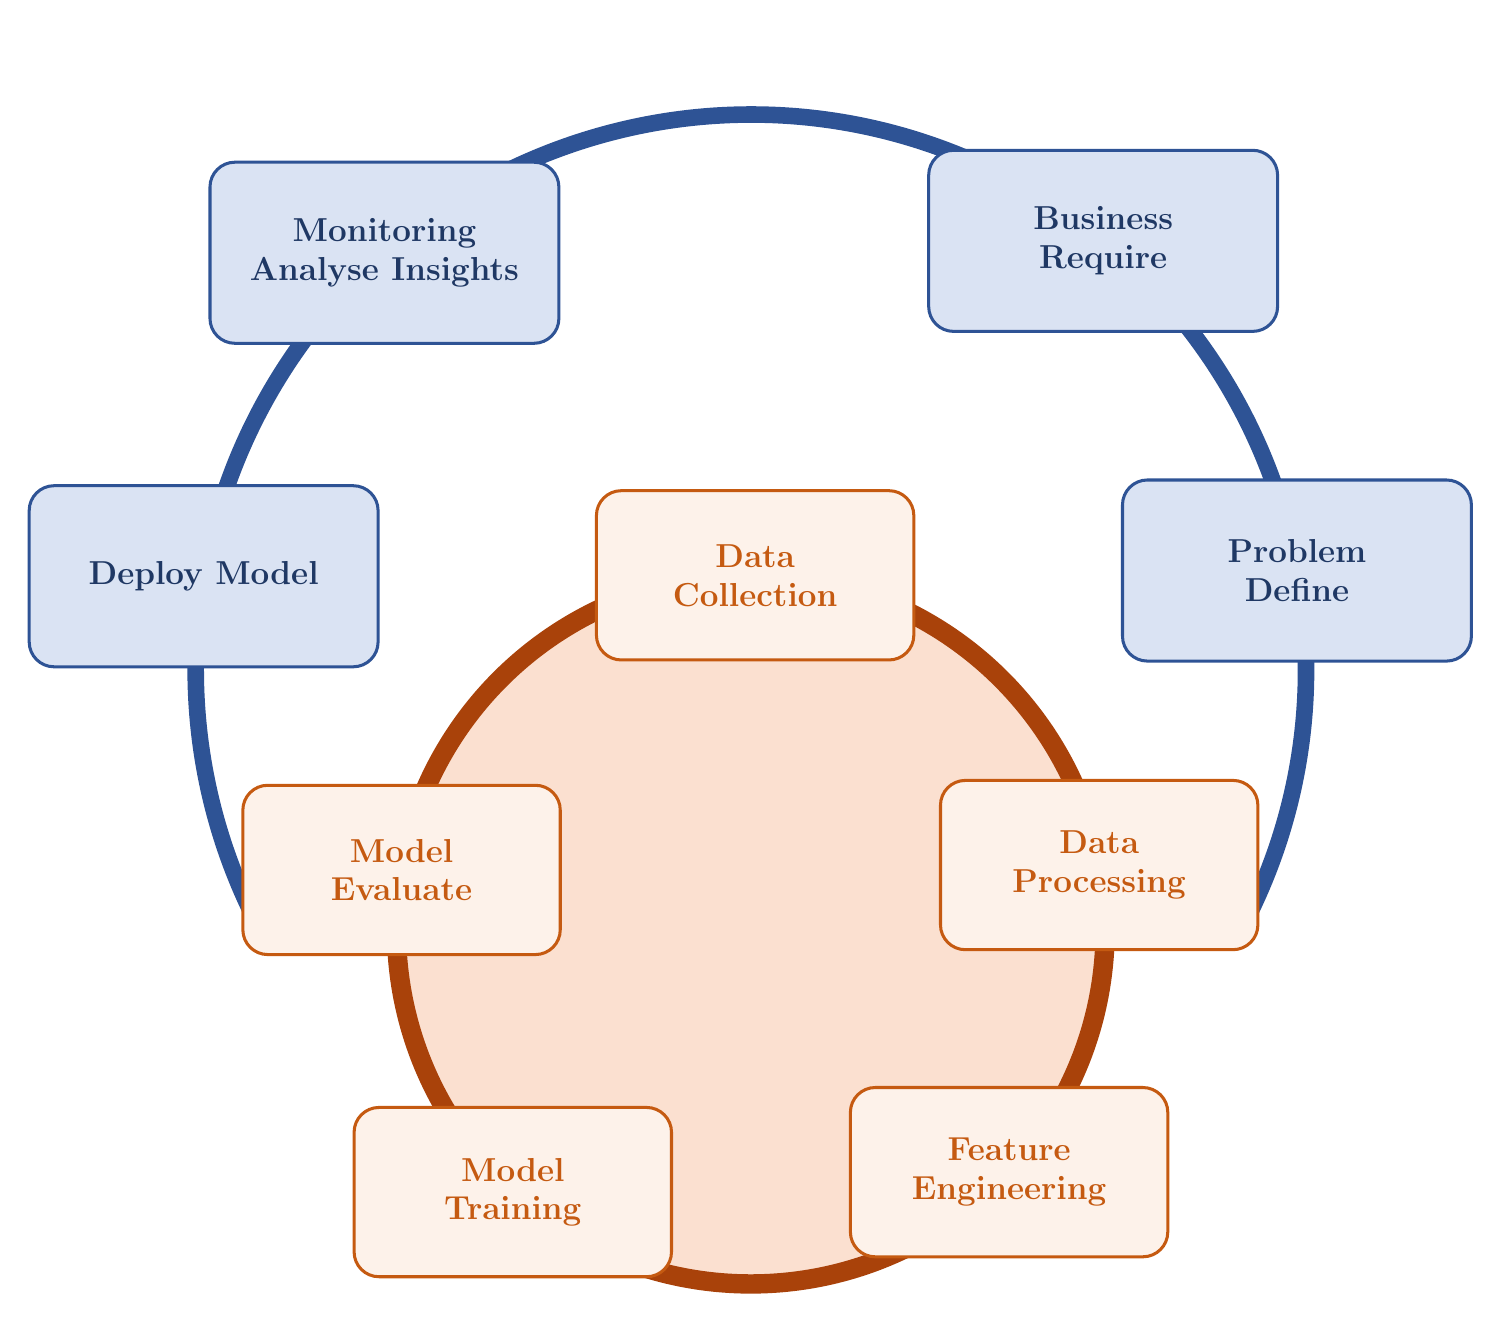
\begin{tikzpicture}[
  hopxanh/.style={
    draw=cXanhVien, line width=1.1pt, fill=cXanhNen, rounded corners=9pt,
    align=center, inner sep=4pt, text width=4.15cm, minimum height=2.3cm,
    font=\large\bfseries, text=cXanhChu
  },
  hopcam/.style={
    draw=cCamVien, line width=1.1pt, fill=cCamHop, rounded corners=9pt,
    align=center, inner sep=4pt, text width=3.75cm, minimum height=2.15cm,
    font=\large\bfseries, text=cCamVien
  }
]

% ── Hai duong tron: tam va ban kinh do tu ban goc ──
% Duong tron xanh : tam (0; 3,30) ban kinh 7,05 cm - chi ve cung tu -12 den 194 do
% Duong tron cam  : tam (0; 0)    ban kinh 4,50 cm - ve tron va to mau
\def\Rx{7.05}   \def\Cy{3.30}
\def\Rc{4.50}

% Dia tron cam ve TRUOC de cung xanh khong bi che
\fill[cCamNen] (0,0) circle (\Rc);
\draw[cCamVong, line width=7pt] (0,0) circle (\Rc);

% Cung tron xanh o ngoai. Hai dau keo den -27 va 207 do de diem cuoi nam HAN vao trong
% hop 'Xu ly du lieu' va 'Danh gia mo hinh'; hop ve sau nen che kin dau cung, nhin ra hai
% vong noi lien nhau dung nhu ban goc. De -12/194 do thi dau cung ho ra ngoai mep hop,
% thanh ra hai net xanh bi cut lung lo.
\draw[cXanhVien, line width=6pt]
  ([shift={(0,\Cy)}]-27:\Rx) arc[start angle=-27, end angle=207, radius=\Rx];

% ── Bon hop tren cung xanh ──
\node[hopxanh] at ($(0,\Cy)+(131.3:\Rx)$) {\Lmonitor};
\node[hopxanh] at ($(0,\Cy)+( 50.6:\Rx)$) {\Lbusiness};
\node[hopxanh] at ($(0,\Cy)+( 10.3:\Rx)$) {\Lproblem};
\node[hopxanh] at ($(0,\Cy)+(170.3:\Rx)$) {\Ldeploy};

% ── Nam hop tren vong cam ──
\node[hopcam] at ( 89.3:\Rc) {\Lcollect};
\node[hopcam] at ( 10.5:\Rc) {\Lprocess};
\node[hopcam] at (-43.2:\Rc) {\Lfeature};
\node[hopcam] at (227.8:\Rc) {\Ltrain};
\node[hopcam] at (170.3:\Rc) {\Levaluate};

\end{tikzpicture}
\end{document}
"
%    xelatex -jobname=sodo_ml_lifecycle_vi "\def\LANGVI{1}% =============================================================================
%  So do VONG DOI HOC MAY (ML Life Cycle) - ve lai tu slide 9 cua tai lieu
%  Data_Version_Control_V3.pdf (AI VIET NAM, All-in-One 2025).
%
%  Ve lai DUNG BO CUC goc: 1 cung tron mau xanh o ngoai mang 4 hop, 1 vong tron
%  to mau cam o trong mang 5 hop. Toa do goc do bang cach do lai vi tri tam va
%  ban kinh hai duong tron tren anh render 150 dpi cua slide, roi doi ra cm.
%
%  KHONG chep logo, tieu de slide, thanh mau va so trang cua tai lieu goc - do la
%  nhan dien thuong hieu cua ho, dua vao luan van se thanh mao nhan. Chi ve lai
%  phan so do.
%
%  Dung lai HAI ban:
%    xelatex -jobname=sodo_ml_lifecycle_en "\def\LANGVI{0}\input{sodo_ml_lifecycle_nguon.tex}"
%    xelatex -jobname=sodo_ml_lifecycle_vi "\def\LANGVI{1}\input{sodo_ml_lifecycle_nguon.tex}"
%
%  GHI CHU: ban goc viet sai chinh ta "Model Traing". Ban ve lai dung
%  "Model Training". Muon giu nguyen loi cua ban goc thi sua lai o \Ltrain.
% =============================================================================
\documentclass[12pt]{article}
\usepackage{fontspec}
\setmainfont{TeX Gyre Termes}          % chu co chan, khop kieu chu ban goc
% Khung giay do vua voi so do: TikZ do duoc 522,2 x 447,7 pt = 18,4 x 15,8 cm,
% cong dong tieu de va le nen cao 18,5 cm thi hinh nam gon 1 trang, khong bi day sang trang 2.
\usepackage[margin=0.5cm,paperwidth=19.5cm,paperheight=18.5cm]{geometry}
\usepackage{tikz}
\usetikzlibrary{arrows.meta,calc}
\pagestyle{empty}

% ── Bang mau lay tu anh render cua slide goc ──
\definecolor{cXanhVien}{HTML}{2E5395}   % vien va cung tron xanh
\definecolor{cXanhNen}{HTML}{DAE3F3}    % nen hop xanh
\definecolor{cXanhChu}{HTML}{1F3864}    % chu trong hop xanh
\definecolor{cCamVien}{HTML}{C55A11}    % vien hop cam va chu cam
\definecolor{cCamVong}{HTML}{A9420A}    % vanh tron cam dam
\definecolor{cCamNen}{HTML}{FBE0D0}     % nen dia tron cam
\definecolor{cCamHop}{HTML}{FDF2EA}     % nen hop cam

% ── Nhan hai ngon ngu ──
\providecommand{\LANGVI}{0}
\ifnum\LANGVI=1
  \def\Ltieude{Vòng đời học máy}
  \def\Lmonitor{Giám sát\\Phân tích thông tin}
  \def\Lbusiness{Yêu cầu\\nghiệp vụ}
  \def\Lproblem{Xác định\\bài toán}
  \def\Ldeploy{Triển khai mô hình}
  \def\Lcollect{Thu thập\\dữ liệu}
  \def\Lprocess{Xử lý\\dữ liệu}
  \def\Lfeature{Sinh\\đặc trưng}
  \def\Ltrain{Huấn luyện\\mô hình}
  \def\Levaluate{Đánh giá\\mô hình}
\else
  \def\Ltieude{ML Life Cycle}
  \def\Lmonitor{Monitoring\\Analyse Insights}
  \def\Lbusiness{Business\\Require}
  \def\Lproblem{Problem\\Define}
  \def\Ldeploy{Deploy Model}
  \def\Lcollect{Data\\Collection}
  \def\Lprocess{Data\\Processing}
  \def\Lfeature{Feature\\Engineering}
  \def\Ltrain{Model\\Training}
  \def\Levaluate{Model\\Evaluate}
\fi

\begin{document}
\noindent{\Large\bfseries\color{cXanhChu}$\diamond$~\Ltieude}\par
\vspace{2mm}
\centering
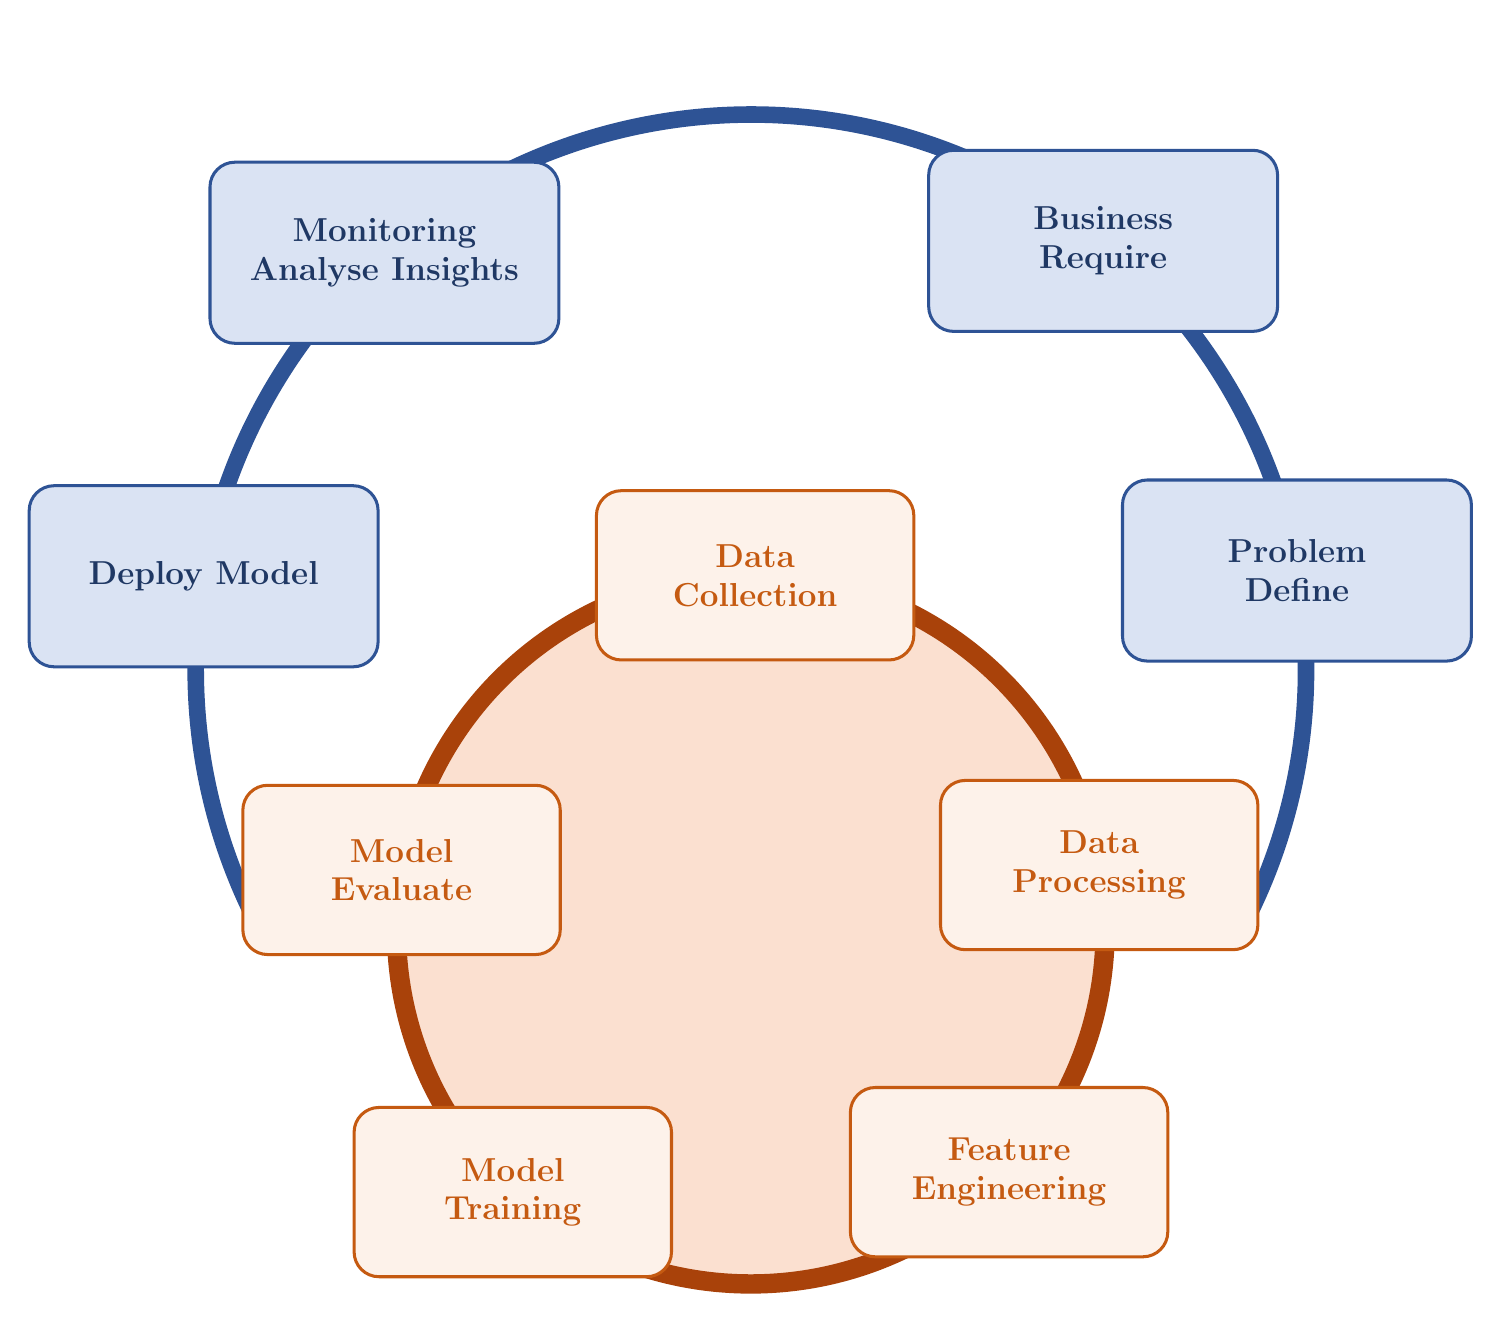
\begin{tikzpicture}[
  hopxanh/.style={
    draw=cXanhVien, line width=1.1pt, fill=cXanhNen, rounded corners=9pt,
    align=center, inner sep=4pt, text width=4.15cm, minimum height=2.3cm,
    font=\large\bfseries, text=cXanhChu
  },
  hopcam/.style={
    draw=cCamVien, line width=1.1pt, fill=cCamHop, rounded corners=9pt,
    align=center, inner sep=4pt, text width=3.75cm, minimum height=2.15cm,
    font=\large\bfseries, text=cCamVien
  }
]

% ── Hai duong tron: tam va ban kinh do tu ban goc ──
% Duong tron xanh : tam (0; 3,30) ban kinh 7,05 cm - chi ve cung tu -12 den 194 do
% Duong tron cam  : tam (0; 0)    ban kinh 4,50 cm - ve tron va to mau
\def\Rx{7.05}   \def\Cy{3.30}
\def\Rc{4.50}

% Dia tron cam ve TRUOC de cung xanh khong bi che
\fill[cCamNen] (0,0) circle (\Rc);
\draw[cCamVong, line width=7pt] (0,0) circle (\Rc);

% Cung tron xanh o ngoai. Hai dau keo den -27 va 207 do de diem cuoi nam HAN vao trong
% hop 'Xu ly du lieu' va 'Danh gia mo hinh'; hop ve sau nen che kin dau cung, nhin ra hai
% vong noi lien nhau dung nhu ban goc. De -12/194 do thi dau cung ho ra ngoai mep hop,
% thanh ra hai net xanh bi cut lung lo.
\draw[cXanhVien, line width=6pt]
  ([shift={(0,\Cy)}]-27:\Rx) arc[start angle=-27, end angle=207, radius=\Rx];

% ── Bon hop tren cung xanh ──
\node[hopxanh] at ($(0,\Cy)+(131.3:\Rx)$) {\Lmonitor};
\node[hopxanh] at ($(0,\Cy)+( 50.6:\Rx)$) {\Lbusiness};
\node[hopxanh] at ($(0,\Cy)+( 10.3:\Rx)$) {\Lproblem};
\node[hopxanh] at ($(0,\Cy)+(170.3:\Rx)$) {\Ldeploy};

% ── Nam hop tren vong cam ──
\node[hopcam] at ( 89.3:\Rc) {\Lcollect};
\node[hopcam] at ( 10.5:\Rc) {\Lprocess};
\node[hopcam] at (-43.2:\Rc) {\Lfeature};
\node[hopcam] at (227.8:\Rc) {\Ltrain};
\node[hopcam] at (170.3:\Rc) {\Levaluate};

\end{tikzpicture}
\end{document}
"
%
%  GHI CHU: ban goc viet sai chinh ta "Model Traing". Ban ve lai dung
%  "Model Training". Muon giu nguyen loi cua ban goc thi sua lai o \Ltrain.
% =============================================================================
\documentclass[12pt]{article}
\usepackage{fontspec}
\setmainfont{TeX Gyre Termes}          % chu co chan, khop kieu chu ban goc
% Khung giay do vua voi so do: TikZ do duoc 522,2 x 447,7 pt = 18,4 x 15,8 cm,
% cong dong tieu de va le nen cao 18,5 cm thi hinh nam gon 1 trang, khong bi day sang trang 2.
\usepackage[margin=0.5cm,paperwidth=19.5cm,paperheight=18.5cm]{geometry}
\usepackage{tikz}
\usetikzlibrary{arrows.meta,calc}
\pagestyle{empty}

% ── Bang mau lay tu anh render cua slide goc ──
\definecolor{cXanhVien}{HTML}{2E5395}   % vien va cung tron xanh
\definecolor{cXanhNen}{HTML}{DAE3F3}    % nen hop xanh
\definecolor{cXanhChu}{HTML}{1F3864}    % chu trong hop xanh
\definecolor{cCamVien}{HTML}{C55A11}    % vien hop cam va chu cam
\definecolor{cCamVong}{HTML}{A9420A}    % vanh tron cam dam
\definecolor{cCamNen}{HTML}{FBE0D0}     % nen dia tron cam
\definecolor{cCamHop}{HTML}{FDF2EA}     % nen hop cam

% ── Nhan hai ngon ngu ──
\providecommand{\LANGVI}{0}
\ifnum\LANGVI=1
  \def\Ltieude{Vòng đời học máy}
  \def\Lmonitor{Giám sát\\Phân tích thông tin}
  \def\Lbusiness{Yêu cầu\\nghiệp vụ}
  \def\Lproblem{Xác định\\bài toán}
  \def\Ldeploy{Triển khai mô hình}
  \def\Lcollect{Thu thập\\dữ liệu}
  \def\Lprocess{Xử lý\\dữ liệu}
  \def\Lfeature{Sinh\\đặc trưng}
  \def\Ltrain{Huấn luyện\\mô hình}
  \def\Levaluate{Đánh giá\\mô hình}
\else
  \def\Ltieude{ML Life Cycle}
  \def\Lmonitor{Monitoring\\Analyse Insights}
  \def\Lbusiness{Business\\Require}
  \def\Lproblem{Problem\\Define}
  \def\Ldeploy{Deploy Model}
  \def\Lcollect{Data\\Collection}
  \def\Lprocess{Data\\Processing}
  \def\Lfeature{Feature\\Engineering}
  \def\Ltrain{Model\\Training}
  \def\Levaluate{Model\\Evaluate}
\fi

\begin{document}
\noindent{\Large\bfseries\color{cXanhChu}$\diamond$~\Ltieude}\par
\vspace{2mm}
\centering
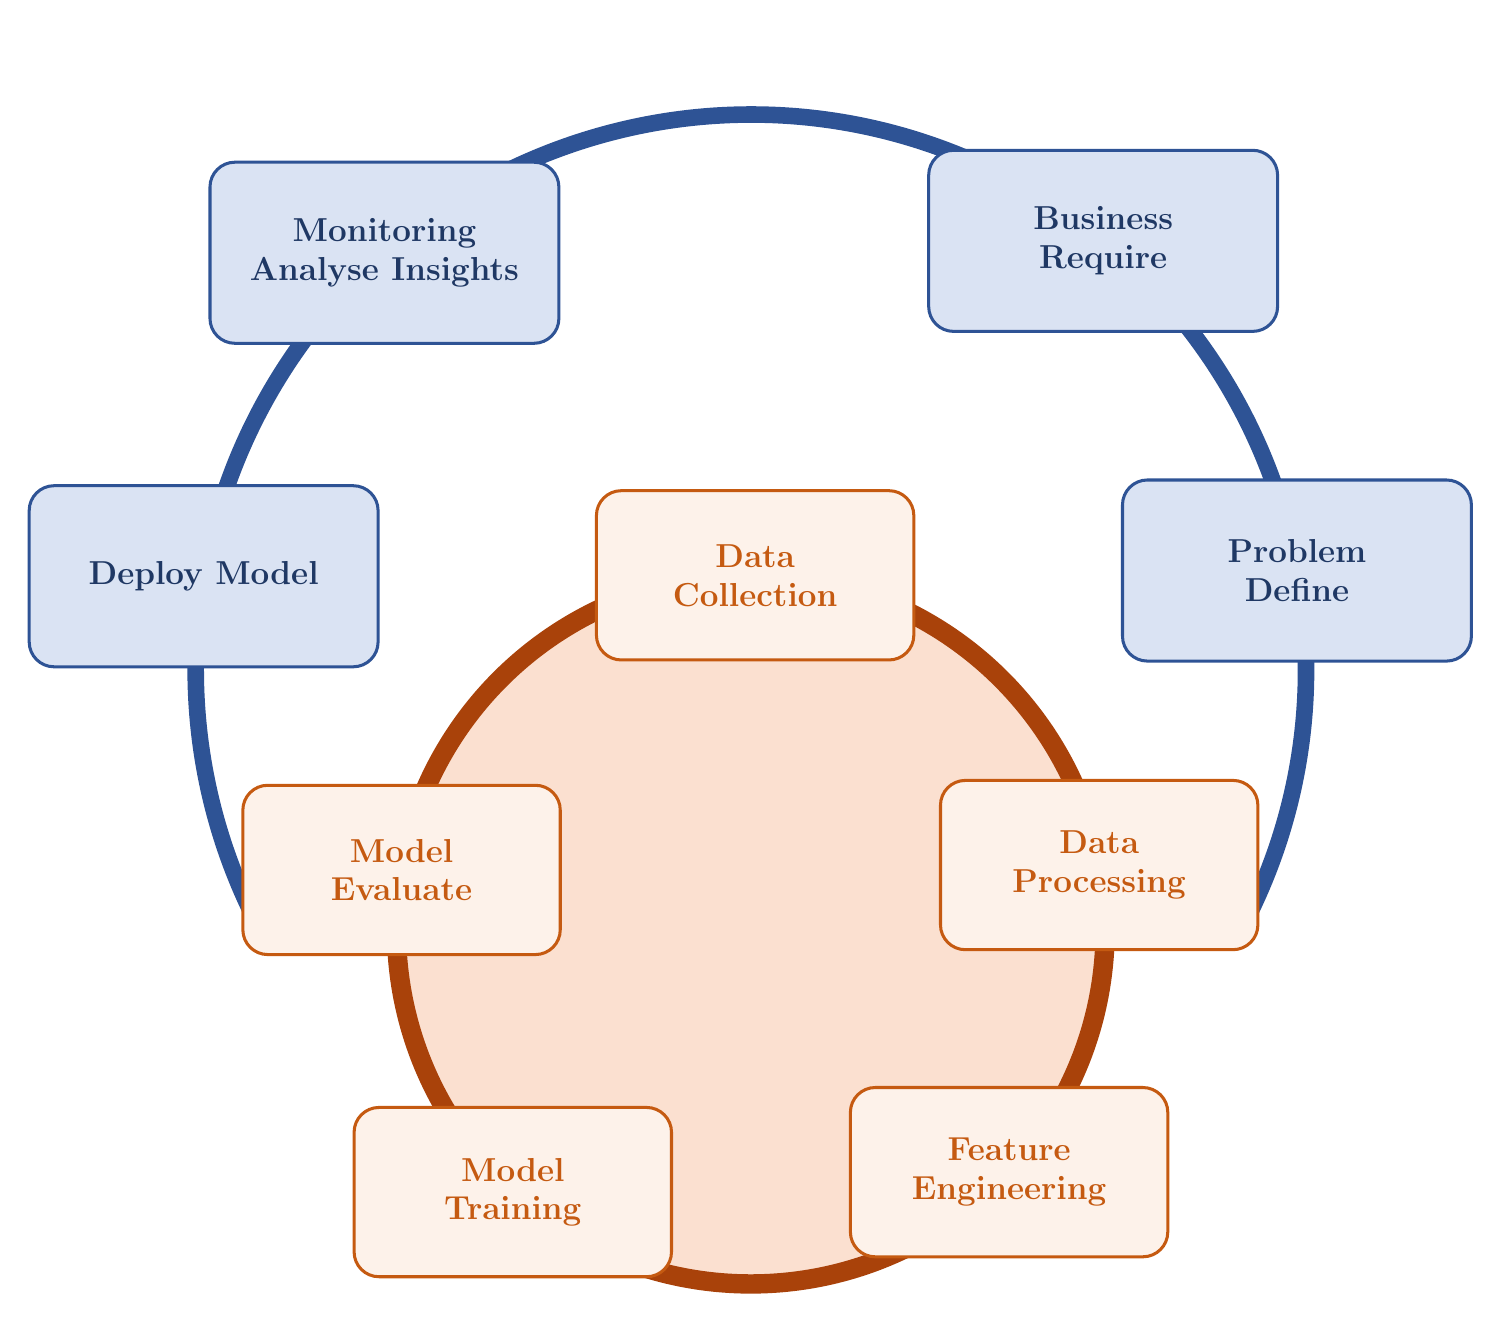
\begin{tikzpicture}[
  hopxanh/.style={
    draw=cXanhVien, line width=1.1pt, fill=cXanhNen, rounded corners=9pt,
    align=center, inner sep=4pt, text width=4.15cm, minimum height=2.3cm,
    font=\large\bfseries, text=cXanhChu
  },
  hopcam/.style={
    draw=cCamVien, line width=1.1pt, fill=cCamHop, rounded corners=9pt,
    align=center, inner sep=4pt, text width=3.75cm, minimum height=2.15cm,
    font=\large\bfseries, text=cCamVien
  }
]

% ── Hai duong tron: tam va ban kinh do tu ban goc ──
% Duong tron xanh : tam (0; 3,30) ban kinh 7,05 cm - chi ve cung tu -12 den 194 do
% Duong tron cam  : tam (0; 0)    ban kinh 4,50 cm - ve tron va to mau
\def\Rx{7.05}   \def\Cy{3.30}
\def\Rc{4.50}

% Dia tron cam ve TRUOC de cung xanh khong bi che
\fill[cCamNen] (0,0) circle (\Rc);
\draw[cCamVong, line width=7pt] (0,0) circle (\Rc);

% Cung tron xanh o ngoai. Hai dau keo den -27 va 207 do de diem cuoi nam HAN vao trong
% hop 'Xu ly du lieu' va 'Danh gia mo hinh'; hop ve sau nen che kin dau cung, nhin ra hai
% vong noi lien nhau dung nhu ban goc. De -12/194 do thi dau cung ho ra ngoai mep hop,
% thanh ra hai net xanh bi cut lung lo.
\draw[cXanhVien, line width=6pt]
  ([shift={(0,\Cy)}]-27:\Rx) arc[start angle=-27, end angle=207, radius=\Rx];

% ── Bon hop tren cung xanh ──
\node[hopxanh] at ($(0,\Cy)+(131.3:\Rx)$) {\Lmonitor};
\node[hopxanh] at ($(0,\Cy)+( 50.6:\Rx)$) {\Lbusiness};
\node[hopxanh] at ($(0,\Cy)+( 10.3:\Rx)$) {\Lproblem};
\node[hopxanh] at ($(0,\Cy)+(170.3:\Rx)$) {\Ldeploy};

% ── Nam hop tren vong cam ──
\node[hopcam] at ( 89.3:\Rc) {\Lcollect};
\node[hopcam] at ( 10.5:\Rc) {\Lprocess};
\node[hopcam] at (-43.2:\Rc) {\Lfeature};
\node[hopcam] at (227.8:\Rc) {\Ltrain};
\node[hopcam] at (170.3:\Rc) {\Levaluate};

\end{tikzpicture}
\end{document}
"
%    xelatex -jobname=sodo_ml_lifecycle_vi "\def\LANGVI{1}% =============================================================================
%  So do VONG DOI HOC MAY (ML Life Cycle) - ve lai tu slide 9 cua tai lieu
%  Data_Version_Control_V3.pdf (AI VIET NAM, All-in-One 2025).
%
%  Ve lai DUNG BO CUC goc: 1 cung tron mau xanh o ngoai mang 4 hop, 1 vong tron
%  to mau cam o trong mang 5 hop. Toa do goc do bang cach do lai vi tri tam va
%  ban kinh hai duong tron tren anh render 150 dpi cua slide, roi doi ra cm.
%
%  KHONG chep logo, tieu de slide, thanh mau va so trang cua tai lieu goc - do la
%  nhan dien thuong hieu cua ho, dua vao luan van se thanh mao nhan. Chi ve lai
%  phan so do.
%
%  Dung lai HAI ban:
%    xelatex -jobname=sodo_ml_lifecycle_en "\def\LANGVI{0}% =============================================================================
%  So do VONG DOI HOC MAY (ML Life Cycle) - ve lai tu slide 9 cua tai lieu
%  Data_Version_Control_V3.pdf (AI VIET NAM, All-in-One 2025).
%
%  Ve lai DUNG BO CUC goc: 1 cung tron mau xanh o ngoai mang 4 hop, 1 vong tron
%  to mau cam o trong mang 5 hop. Toa do goc do bang cach do lai vi tri tam va
%  ban kinh hai duong tron tren anh render 150 dpi cua slide, roi doi ra cm.
%
%  KHONG chep logo, tieu de slide, thanh mau va so trang cua tai lieu goc - do la
%  nhan dien thuong hieu cua ho, dua vao luan van se thanh mao nhan. Chi ve lai
%  phan so do.
%
%  Dung lai HAI ban:
%    xelatex -jobname=sodo_ml_lifecycle_en "\def\LANGVI{0}\input{sodo_ml_lifecycle_nguon.tex}"
%    xelatex -jobname=sodo_ml_lifecycle_vi "\def\LANGVI{1}\input{sodo_ml_lifecycle_nguon.tex}"
%
%  GHI CHU: ban goc viet sai chinh ta "Model Traing". Ban ve lai dung
%  "Model Training". Muon giu nguyen loi cua ban goc thi sua lai o \Ltrain.
% =============================================================================
\documentclass[12pt]{article}
\usepackage{fontspec}
\setmainfont{TeX Gyre Termes}          % chu co chan, khop kieu chu ban goc
% Khung giay do vua voi so do: TikZ do duoc 522,2 x 447,7 pt = 18,4 x 15,8 cm,
% cong dong tieu de va le nen cao 18,5 cm thi hinh nam gon 1 trang, khong bi day sang trang 2.
\usepackage[margin=0.5cm,paperwidth=19.5cm,paperheight=18.5cm]{geometry}
\usepackage{tikz}
\usetikzlibrary{arrows.meta,calc}
\pagestyle{empty}

% ── Bang mau lay tu anh render cua slide goc ──
\definecolor{cXanhVien}{HTML}{2E5395}   % vien va cung tron xanh
\definecolor{cXanhNen}{HTML}{DAE3F3}    % nen hop xanh
\definecolor{cXanhChu}{HTML}{1F3864}    % chu trong hop xanh
\definecolor{cCamVien}{HTML}{C55A11}    % vien hop cam va chu cam
\definecolor{cCamVong}{HTML}{A9420A}    % vanh tron cam dam
\definecolor{cCamNen}{HTML}{FBE0D0}     % nen dia tron cam
\definecolor{cCamHop}{HTML}{FDF2EA}     % nen hop cam

% ── Nhan hai ngon ngu ──
\providecommand{\LANGVI}{0}
\ifnum\LANGVI=1
  \def\Ltieude{Vòng đời học máy}
  \def\Lmonitor{Giám sát\\Phân tích thông tin}
  \def\Lbusiness{Yêu cầu\\nghiệp vụ}
  \def\Lproblem{Xác định\\bài toán}
  \def\Ldeploy{Triển khai mô hình}
  \def\Lcollect{Thu thập\\dữ liệu}
  \def\Lprocess{Xử lý\\dữ liệu}
  \def\Lfeature{Sinh\\đặc trưng}
  \def\Ltrain{Huấn luyện\\mô hình}
  \def\Levaluate{Đánh giá\\mô hình}
\else
  \def\Ltieude{ML Life Cycle}
  \def\Lmonitor{Monitoring\\Analyse Insights}
  \def\Lbusiness{Business\\Require}
  \def\Lproblem{Problem\\Define}
  \def\Ldeploy{Deploy Model}
  \def\Lcollect{Data\\Collection}
  \def\Lprocess{Data\\Processing}
  \def\Lfeature{Feature\\Engineering}
  \def\Ltrain{Model\\Training}
  \def\Levaluate{Model\\Evaluate}
\fi

\begin{document}
\noindent{\Large\bfseries\color{cXanhChu}$\diamond$~\Ltieude}\par
\vspace{2mm}
\centering
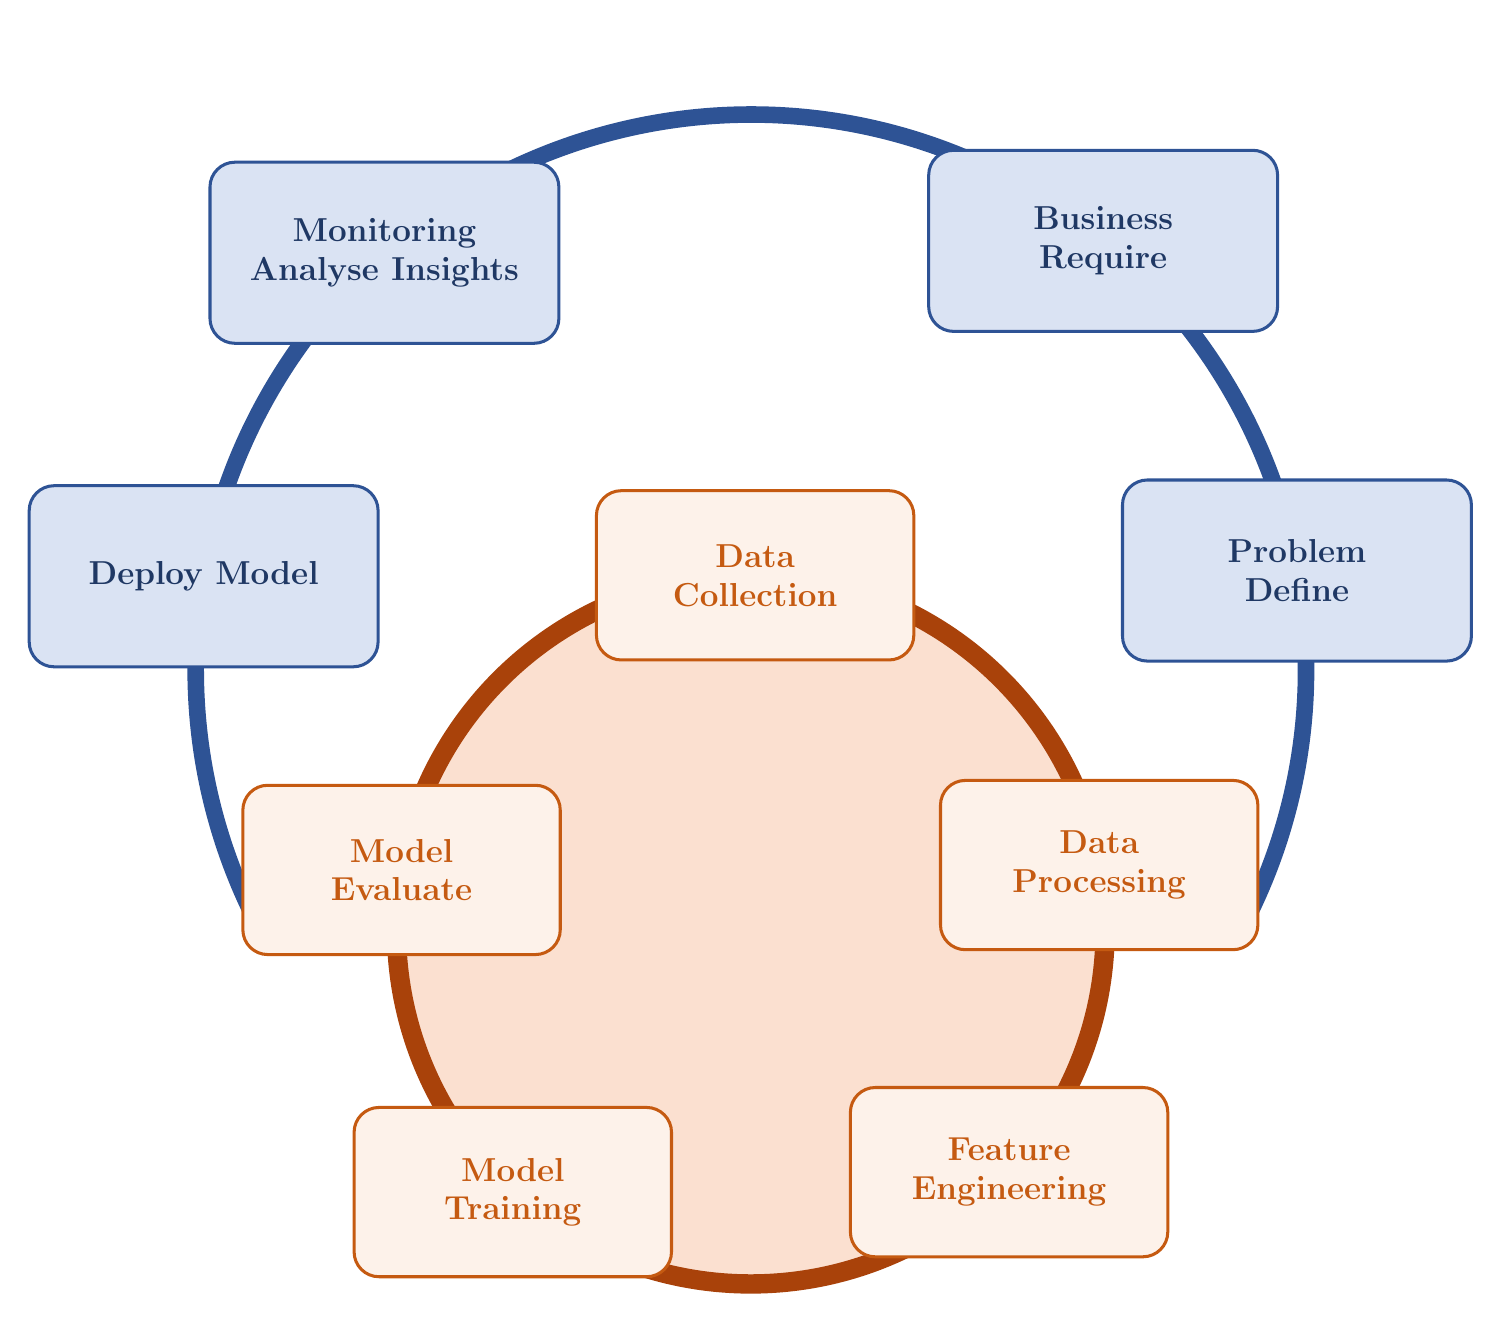
\begin{tikzpicture}[
  hopxanh/.style={
    draw=cXanhVien, line width=1.1pt, fill=cXanhNen, rounded corners=9pt,
    align=center, inner sep=4pt, text width=4.15cm, minimum height=2.3cm,
    font=\large\bfseries, text=cXanhChu
  },
  hopcam/.style={
    draw=cCamVien, line width=1.1pt, fill=cCamHop, rounded corners=9pt,
    align=center, inner sep=4pt, text width=3.75cm, minimum height=2.15cm,
    font=\large\bfseries, text=cCamVien
  }
]

% ── Hai duong tron: tam va ban kinh do tu ban goc ──
% Duong tron xanh : tam (0; 3,30) ban kinh 7,05 cm - chi ve cung tu -12 den 194 do
% Duong tron cam  : tam (0; 0)    ban kinh 4,50 cm - ve tron va to mau
\def\Rx{7.05}   \def\Cy{3.30}
\def\Rc{4.50}

% Dia tron cam ve TRUOC de cung xanh khong bi che
\fill[cCamNen] (0,0) circle (\Rc);
\draw[cCamVong, line width=7pt] (0,0) circle (\Rc);

% Cung tron xanh o ngoai. Hai dau keo den -27 va 207 do de diem cuoi nam HAN vao trong
% hop 'Xu ly du lieu' va 'Danh gia mo hinh'; hop ve sau nen che kin dau cung, nhin ra hai
% vong noi lien nhau dung nhu ban goc. De -12/194 do thi dau cung ho ra ngoai mep hop,
% thanh ra hai net xanh bi cut lung lo.
\draw[cXanhVien, line width=6pt]
  ([shift={(0,\Cy)}]-27:\Rx) arc[start angle=-27, end angle=207, radius=\Rx];

% ── Bon hop tren cung xanh ──
\node[hopxanh] at ($(0,\Cy)+(131.3:\Rx)$) {\Lmonitor};
\node[hopxanh] at ($(0,\Cy)+( 50.6:\Rx)$) {\Lbusiness};
\node[hopxanh] at ($(0,\Cy)+( 10.3:\Rx)$) {\Lproblem};
\node[hopxanh] at ($(0,\Cy)+(170.3:\Rx)$) {\Ldeploy};

% ── Nam hop tren vong cam ──
\node[hopcam] at ( 89.3:\Rc) {\Lcollect};
\node[hopcam] at ( 10.5:\Rc) {\Lprocess};
\node[hopcam] at (-43.2:\Rc) {\Lfeature};
\node[hopcam] at (227.8:\Rc) {\Ltrain};
\node[hopcam] at (170.3:\Rc) {\Levaluate};

\end{tikzpicture}
\end{document}
"
%    xelatex -jobname=sodo_ml_lifecycle_vi "\def\LANGVI{1}% =============================================================================
%  So do VONG DOI HOC MAY (ML Life Cycle) - ve lai tu slide 9 cua tai lieu
%  Data_Version_Control_V3.pdf (AI VIET NAM, All-in-One 2025).
%
%  Ve lai DUNG BO CUC goc: 1 cung tron mau xanh o ngoai mang 4 hop, 1 vong tron
%  to mau cam o trong mang 5 hop. Toa do goc do bang cach do lai vi tri tam va
%  ban kinh hai duong tron tren anh render 150 dpi cua slide, roi doi ra cm.
%
%  KHONG chep logo, tieu de slide, thanh mau va so trang cua tai lieu goc - do la
%  nhan dien thuong hieu cua ho, dua vao luan van se thanh mao nhan. Chi ve lai
%  phan so do.
%
%  Dung lai HAI ban:
%    xelatex -jobname=sodo_ml_lifecycle_en "\def\LANGVI{0}\input{sodo_ml_lifecycle_nguon.tex}"
%    xelatex -jobname=sodo_ml_lifecycle_vi "\def\LANGVI{1}\input{sodo_ml_lifecycle_nguon.tex}"
%
%  GHI CHU: ban goc viet sai chinh ta "Model Traing". Ban ve lai dung
%  "Model Training". Muon giu nguyen loi cua ban goc thi sua lai o \Ltrain.
% =============================================================================
\documentclass[12pt]{article}
\usepackage{fontspec}
\setmainfont{TeX Gyre Termes}          % chu co chan, khop kieu chu ban goc
% Khung giay do vua voi so do: TikZ do duoc 522,2 x 447,7 pt = 18,4 x 15,8 cm,
% cong dong tieu de va le nen cao 18,5 cm thi hinh nam gon 1 trang, khong bi day sang trang 2.
\usepackage[margin=0.5cm,paperwidth=19.5cm,paperheight=18.5cm]{geometry}
\usepackage{tikz}
\usetikzlibrary{arrows.meta,calc}
\pagestyle{empty}

% ── Bang mau lay tu anh render cua slide goc ──
\definecolor{cXanhVien}{HTML}{2E5395}   % vien va cung tron xanh
\definecolor{cXanhNen}{HTML}{DAE3F3}    % nen hop xanh
\definecolor{cXanhChu}{HTML}{1F3864}    % chu trong hop xanh
\definecolor{cCamVien}{HTML}{C55A11}    % vien hop cam va chu cam
\definecolor{cCamVong}{HTML}{A9420A}    % vanh tron cam dam
\definecolor{cCamNen}{HTML}{FBE0D0}     % nen dia tron cam
\definecolor{cCamHop}{HTML}{FDF2EA}     % nen hop cam

% ── Nhan hai ngon ngu ──
\providecommand{\LANGVI}{0}
\ifnum\LANGVI=1
  \def\Ltieude{Vòng đời học máy}
  \def\Lmonitor{Giám sát\\Phân tích thông tin}
  \def\Lbusiness{Yêu cầu\\nghiệp vụ}
  \def\Lproblem{Xác định\\bài toán}
  \def\Ldeploy{Triển khai mô hình}
  \def\Lcollect{Thu thập\\dữ liệu}
  \def\Lprocess{Xử lý\\dữ liệu}
  \def\Lfeature{Sinh\\đặc trưng}
  \def\Ltrain{Huấn luyện\\mô hình}
  \def\Levaluate{Đánh giá\\mô hình}
\else
  \def\Ltieude{ML Life Cycle}
  \def\Lmonitor{Monitoring\\Analyse Insights}
  \def\Lbusiness{Business\\Require}
  \def\Lproblem{Problem\\Define}
  \def\Ldeploy{Deploy Model}
  \def\Lcollect{Data\\Collection}
  \def\Lprocess{Data\\Processing}
  \def\Lfeature{Feature\\Engineering}
  \def\Ltrain{Model\\Training}
  \def\Levaluate{Model\\Evaluate}
\fi

\begin{document}
\noindent{\Large\bfseries\color{cXanhChu}$\diamond$~\Ltieude}\par
\vspace{2mm}
\centering
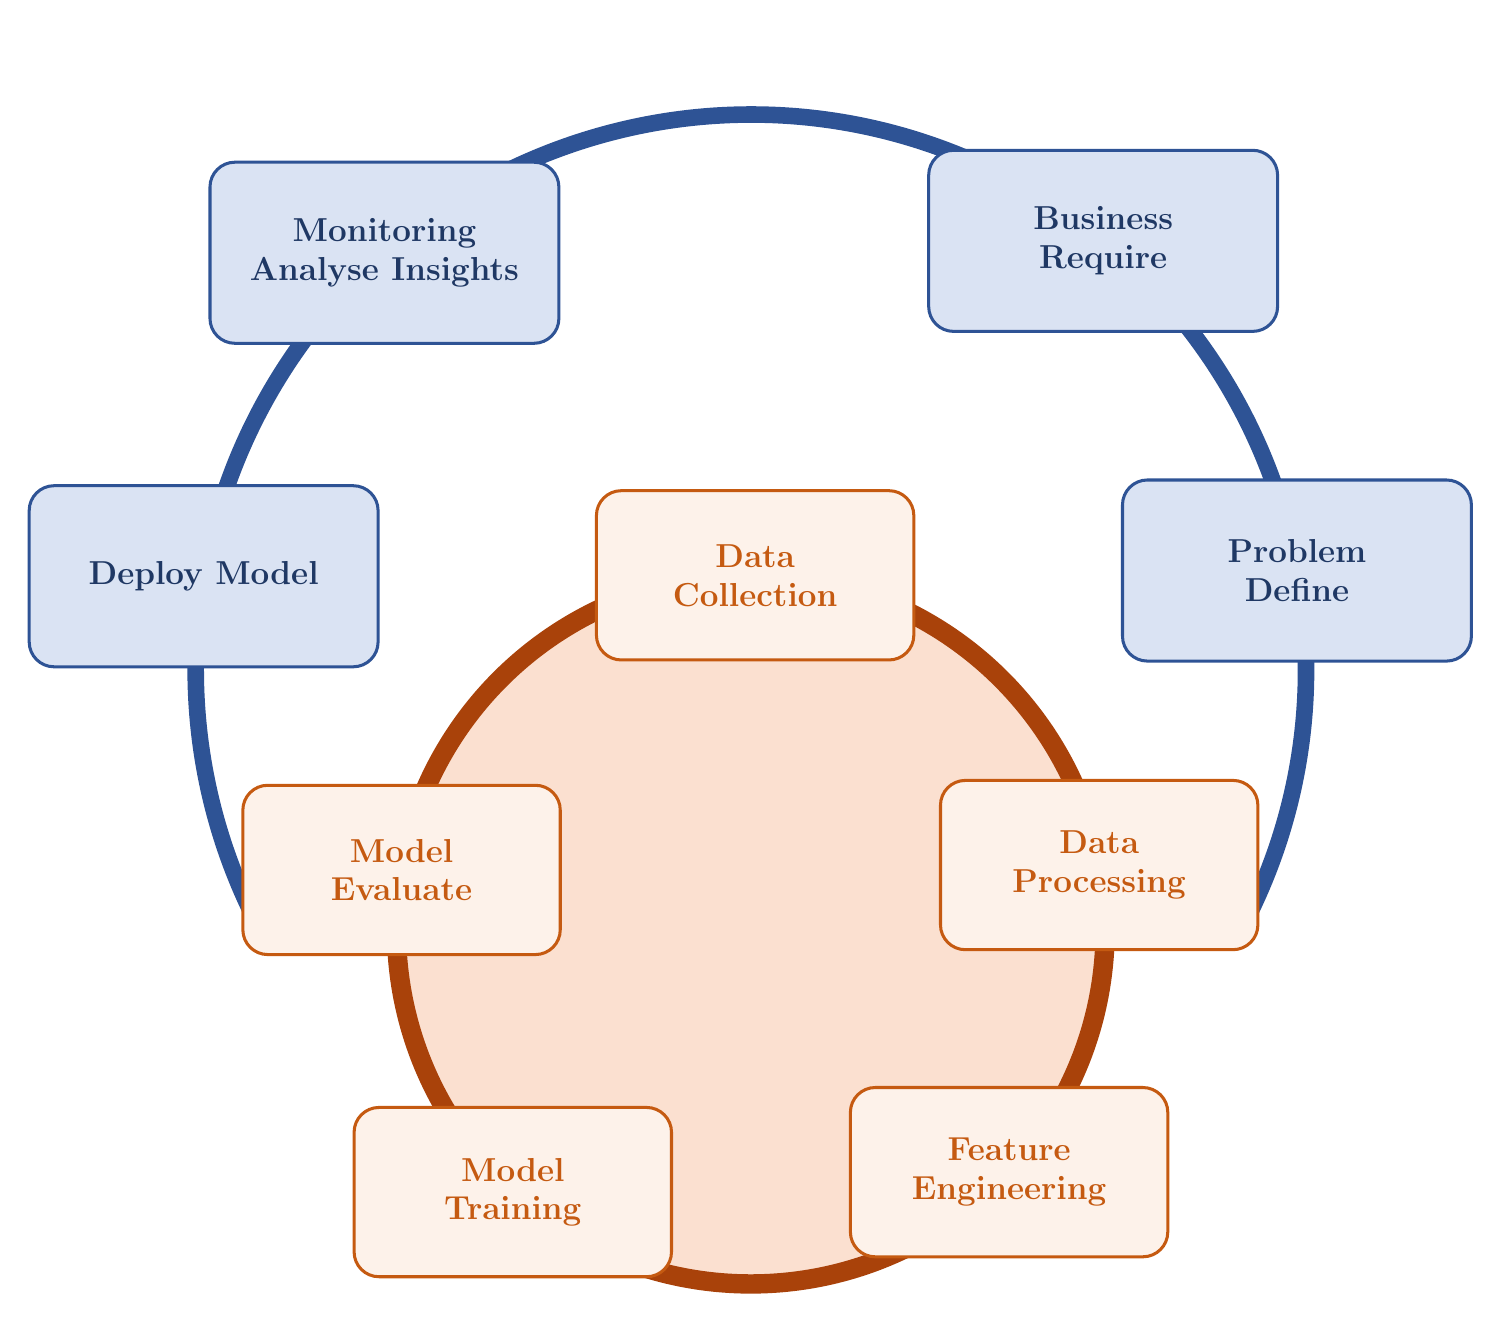
\begin{tikzpicture}[
  hopxanh/.style={
    draw=cXanhVien, line width=1.1pt, fill=cXanhNen, rounded corners=9pt,
    align=center, inner sep=4pt, text width=4.15cm, minimum height=2.3cm,
    font=\large\bfseries, text=cXanhChu
  },
  hopcam/.style={
    draw=cCamVien, line width=1.1pt, fill=cCamHop, rounded corners=9pt,
    align=center, inner sep=4pt, text width=3.75cm, minimum height=2.15cm,
    font=\large\bfseries, text=cCamVien
  }
]

% ── Hai duong tron: tam va ban kinh do tu ban goc ──
% Duong tron xanh : tam (0; 3,30) ban kinh 7,05 cm - chi ve cung tu -12 den 194 do
% Duong tron cam  : tam (0; 0)    ban kinh 4,50 cm - ve tron va to mau
\def\Rx{7.05}   \def\Cy{3.30}
\def\Rc{4.50}

% Dia tron cam ve TRUOC de cung xanh khong bi che
\fill[cCamNen] (0,0) circle (\Rc);
\draw[cCamVong, line width=7pt] (0,0) circle (\Rc);

% Cung tron xanh o ngoai. Hai dau keo den -27 va 207 do de diem cuoi nam HAN vao trong
% hop 'Xu ly du lieu' va 'Danh gia mo hinh'; hop ve sau nen che kin dau cung, nhin ra hai
% vong noi lien nhau dung nhu ban goc. De -12/194 do thi dau cung ho ra ngoai mep hop,
% thanh ra hai net xanh bi cut lung lo.
\draw[cXanhVien, line width=6pt]
  ([shift={(0,\Cy)}]-27:\Rx) arc[start angle=-27, end angle=207, radius=\Rx];

% ── Bon hop tren cung xanh ──
\node[hopxanh] at ($(0,\Cy)+(131.3:\Rx)$) {\Lmonitor};
\node[hopxanh] at ($(0,\Cy)+( 50.6:\Rx)$) {\Lbusiness};
\node[hopxanh] at ($(0,\Cy)+( 10.3:\Rx)$) {\Lproblem};
\node[hopxanh] at ($(0,\Cy)+(170.3:\Rx)$) {\Ldeploy};

% ── Nam hop tren vong cam ──
\node[hopcam] at ( 89.3:\Rc) {\Lcollect};
\node[hopcam] at ( 10.5:\Rc) {\Lprocess};
\node[hopcam] at (-43.2:\Rc) {\Lfeature};
\node[hopcam] at (227.8:\Rc) {\Ltrain};
\node[hopcam] at (170.3:\Rc) {\Levaluate};

\end{tikzpicture}
\end{document}
"
%
%  GHI CHU: ban goc viet sai chinh ta "Model Traing". Ban ve lai dung
%  "Model Training". Muon giu nguyen loi cua ban goc thi sua lai o \Ltrain.
% =============================================================================
\documentclass[12pt]{article}
\usepackage{fontspec}
\setmainfont{TeX Gyre Termes}          % chu co chan, khop kieu chu ban goc
% Khung giay do vua voi so do: TikZ do duoc 522,2 x 447,7 pt = 18,4 x 15,8 cm,
% cong dong tieu de va le nen cao 18,5 cm thi hinh nam gon 1 trang, khong bi day sang trang 2.
\usepackage[margin=0.5cm,paperwidth=19.5cm,paperheight=18.5cm]{geometry}
\usepackage{tikz}
\usetikzlibrary{arrows.meta,calc}
\pagestyle{empty}

% ── Bang mau lay tu anh render cua slide goc ──
\definecolor{cXanhVien}{HTML}{2E5395}   % vien va cung tron xanh
\definecolor{cXanhNen}{HTML}{DAE3F3}    % nen hop xanh
\definecolor{cXanhChu}{HTML}{1F3864}    % chu trong hop xanh
\definecolor{cCamVien}{HTML}{C55A11}    % vien hop cam va chu cam
\definecolor{cCamVong}{HTML}{A9420A}    % vanh tron cam dam
\definecolor{cCamNen}{HTML}{FBE0D0}     % nen dia tron cam
\definecolor{cCamHop}{HTML}{FDF2EA}     % nen hop cam

% ── Nhan hai ngon ngu ──
\providecommand{\LANGVI}{0}
\ifnum\LANGVI=1
  \def\Ltieude{Vòng đời học máy}
  \def\Lmonitor{Giám sát\\Phân tích thông tin}
  \def\Lbusiness{Yêu cầu\\nghiệp vụ}
  \def\Lproblem{Xác định\\bài toán}
  \def\Ldeploy{Triển khai mô hình}
  \def\Lcollect{Thu thập\\dữ liệu}
  \def\Lprocess{Xử lý\\dữ liệu}
  \def\Lfeature{Sinh\\đặc trưng}
  \def\Ltrain{Huấn luyện\\mô hình}
  \def\Levaluate{Đánh giá\\mô hình}
\else
  \def\Ltieude{ML Life Cycle}
  \def\Lmonitor{Monitoring\\Analyse Insights}
  \def\Lbusiness{Business\\Require}
  \def\Lproblem{Problem\\Define}
  \def\Ldeploy{Deploy Model}
  \def\Lcollect{Data\\Collection}
  \def\Lprocess{Data\\Processing}
  \def\Lfeature{Feature\\Engineering}
  \def\Ltrain{Model\\Training}
  \def\Levaluate{Model\\Evaluate}
\fi

\begin{document}
\noindent{\Large\bfseries\color{cXanhChu}$\diamond$~\Ltieude}\par
\vspace{2mm}
\centering
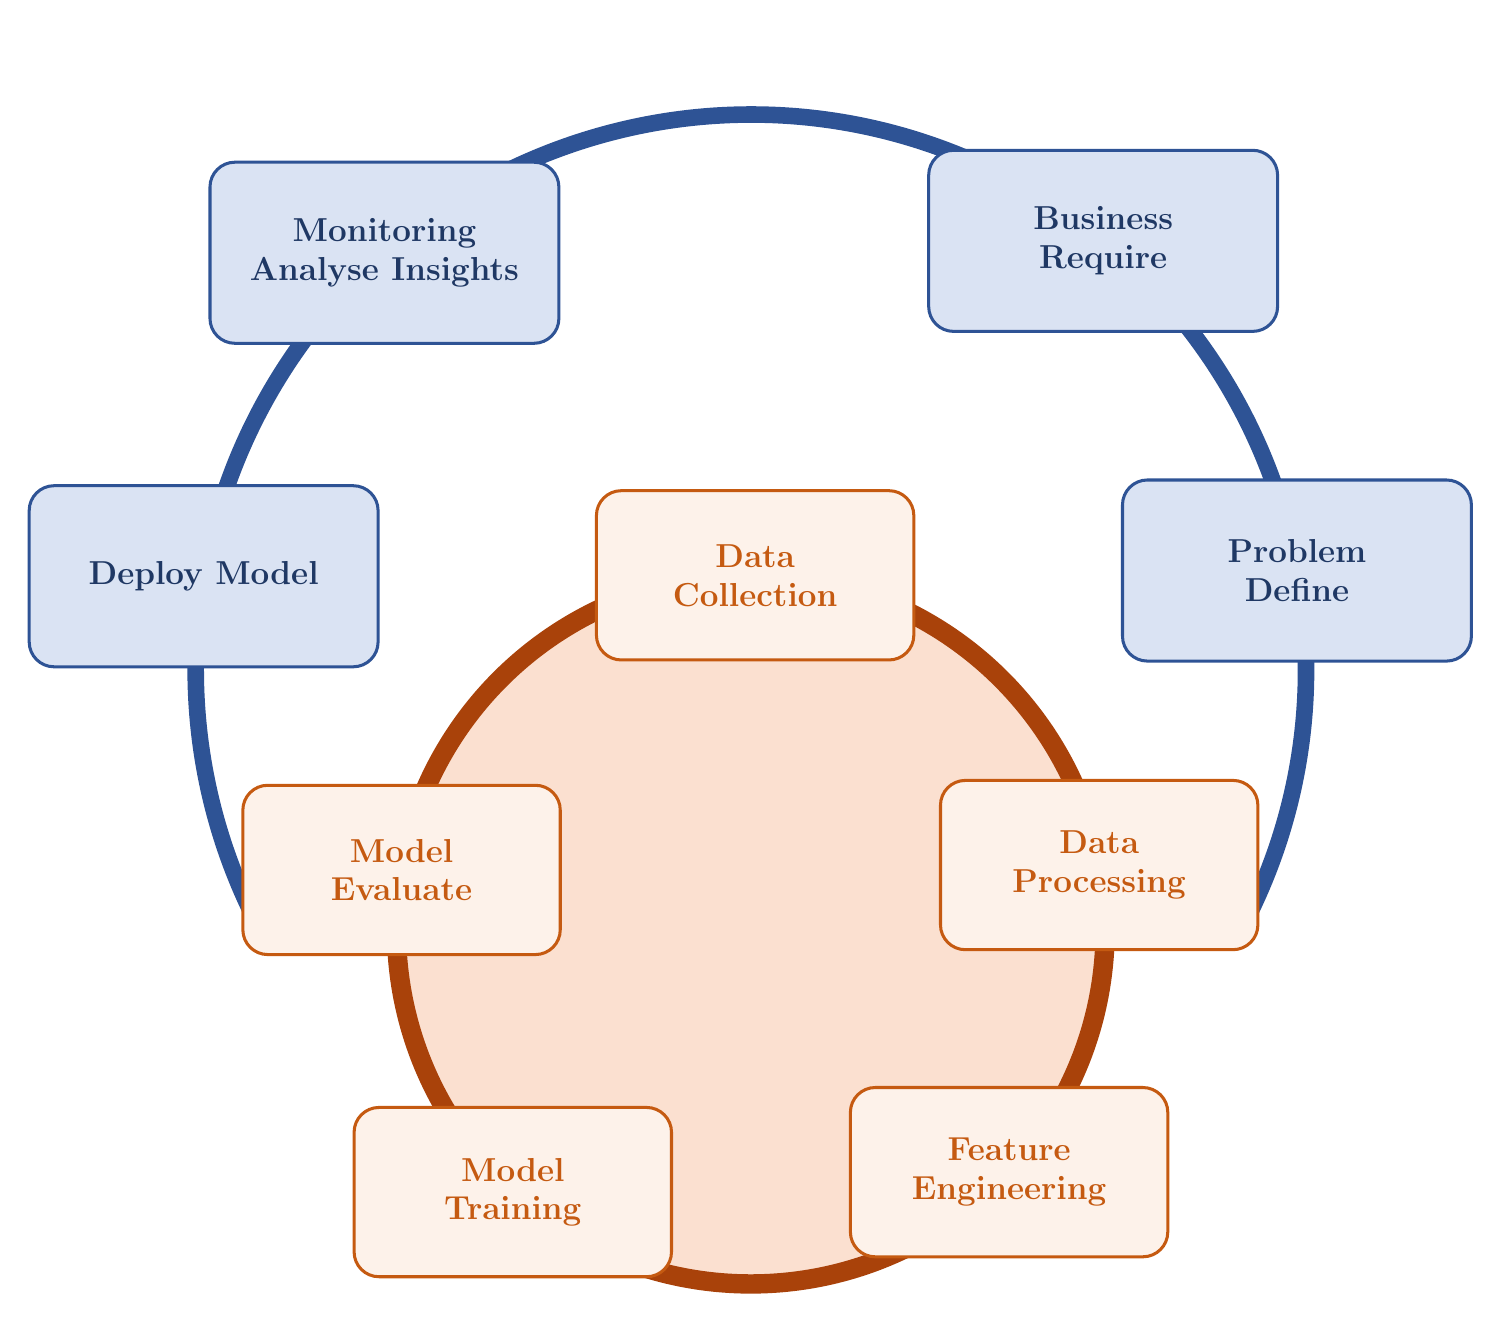
\begin{tikzpicture}[
  hopxanh/.style={
    draw=cXanhVien, line width=1.1pt, fill=cXanhNen, rounded corners=9pt,
    align=center, inner sep=4pt, text width=4.15cm, minimum height=2.3cm,
    font=\large\bfseries, text=cXanhChu
  },
  hopcam/.style={
    draw=cCamVien, line width=1.1pt, fill=cCamHop, rounded corners=9pt,
    align=center, inner sep=4pt, text width=3.75cm, minimum height=2.15cm,
    font=\large\bfseries, text=cCamVien
  }
]

% ── Hai duong tron: tam va ban kinh do tu ban goc ──
% Duong tron xanh : tam (0; 3,30) ban kinh 7,05 cm - chi ve cung tu -12 den 194 do
% Duong tron cam  : tam (0; 0)    ban kinh 4,50 cm - ve tron va to mau
\def\Rx{7.05}   \def\Cy{3.30}
\def\Rc{4.50}

% Dia tron cam ve TRUOC de cung xanh khong bi che
\fill[cCamNen] (0,0) circle (\Rc);
\draw[cCamVong, line width=7pt] (0,0) circle (\Rc);

% Cung tron xanh o ngoai. Hai dau keo den -27 va 207 do de diem cuoi nam HAN vao trong
% hop 'Xu ly du lieu' va 'Danh gia mo hinh'; hop ve sau nen che kin dau cung, nhin ra hai
% vong noi lien nhau dung nhu ban goc. De -12/194 do thi dau cung ho ra ngoai mep hop,
% thanh ra hai net xanh bi cut lung lo.
\draw[cXanhVien, line width=6pt]
  ([shift={(0,\Cy)}]-27:\Rx) arc[start angle=-27, end angle=207, radius=\Rx];

% ── Bon hop tren cung xanh ──
\node[hopxanh] at ($(0,\Cy)+(131.3:\Rx)$) {\Lmonitor};
\node[hopxanh] at ($(0,\Cy)+( 50.6:\Rx)$) {\Lbusiness};
\node[hopxanh] at ($(0,\Cy)+( 10.3:\Rx)$) {\Lproblem};
\node[hopxanh] at ($(0,\Cy)+(170.3:\Rx)$) {\Ldeploy};

% ── Nam hop tren vong cam ──
\node[hopcam] at ( 89.3:\Rc) {\Lcollect};
\node[hopcam] at ( 10.5:\Rc) {\Lprocess};
\node[hopcam] at (-43.2:\Rc) {\Lfeature};
\node[hopcam] at (227.8:\Rc) {\Ltrain};
\node[hopcam] at (170.3:\Rc) {\Levaluate};

\end{tikzpicture}
\end{document}
"
%
%  GHI CHU: ban goc viet sai chinh ta "Model Traing". Ban ve lai dung
%  "Model Training". Muon giu nguyen loi cua ban goc thi sua lai o \Ltrain.
% =============================================================================
\documentclass[12pt]{article}
\usepackage{fontspec}
\setmainfont{TeX Gyre Termes}          % chu co chan, khop kieu chu ban goc
% Khung giay do vua voi so do: TikZ do duoc 522,2 x 447,7 pt = 18,4 x 15,8 cm,
% cong dong tieu de va le nen cao 18,5 cm thi hinh nam gon 1 trang, khong bi day sang trang 2.
\usepackage[margin=0.5cm,paperwidth=19.5cm,paperheight=18.5cm]{geometry}
\usepackage{tikz}
\usetikzlibrary{arrows.meta,calc}
\pagestyle{empty}

% ── Bang mau lay tu anh render cua slide goc ──
\definecolor{cXanhVien}{HTML}{2E5395}   % vien va cung tron xanh
\definecolor{cXanhNen}{HTML}{DAE3F3}    % nen hop xanh
\definecolor{cXanhChu}{HTML}{1F3864}    % chu trong hop xanh
\definecolor{cCamVien}{HTML}{C55A11}    % vien hop cam va chu cam
\definecolor{cCamVong}{HTML}{A9420A}    % vanh tron cam dam
\definecolor{cCamNen}{HTML}{FBE0D0}     % nen dia tron cam
\definecolor{cCamHop}{HTML}{FDF2EA}     % nen hop cam

% ── Nhan hai ngon ngu ──
\providecommand{\LANGVI}{0}
\ifnum\LANGVI=1
  \def\Ltieude{Vòng đời học máy}
  \def\Lmonitor{Giám sát\\Phân tích thông tin}
  \def\Lbusiness{Yêu cầu\\nghiệp vụ}
  \def\Lproblem{Xác định\\bài toán}
  \def\Ldeploy{Triển khai mô hình}
  \def\Lcollect{Thu thập\\dữ liệu}
  \def\Lprocess{Xử lý\\dữ liệu}
  \def\Lfeature{Sinh\\đặc trưng}
  \def\Ltrain{Huấn luyện\\mô hình}
  \def\Levaluate{Đánh giá\\mô hình}
\else
  \def\Ltieude{ML Life Cycle}
  \def\Lmonitor{Monitoring\\Analyse Insights}
  \def\Lbusiness{Business\\Require}
  \def\Lproblem{Problem\\Define}
  \def\Ldeploy{Deploy Model}
  \def\Lcollect{Data\\Collection}
  \def\Lprocess{Data\\Processing}
  \def\Lfeature{Feature\\Engineering}
  \def\Ltrain{Model\\Training}
  \def\Levaluate{Model\\Evaluate}
\fi

\begin{document}
\noindent{\Large\bfseries\color{cXanhChu}$\diamond$~\Ltieude}\par
\vspace{2mm}
\centering
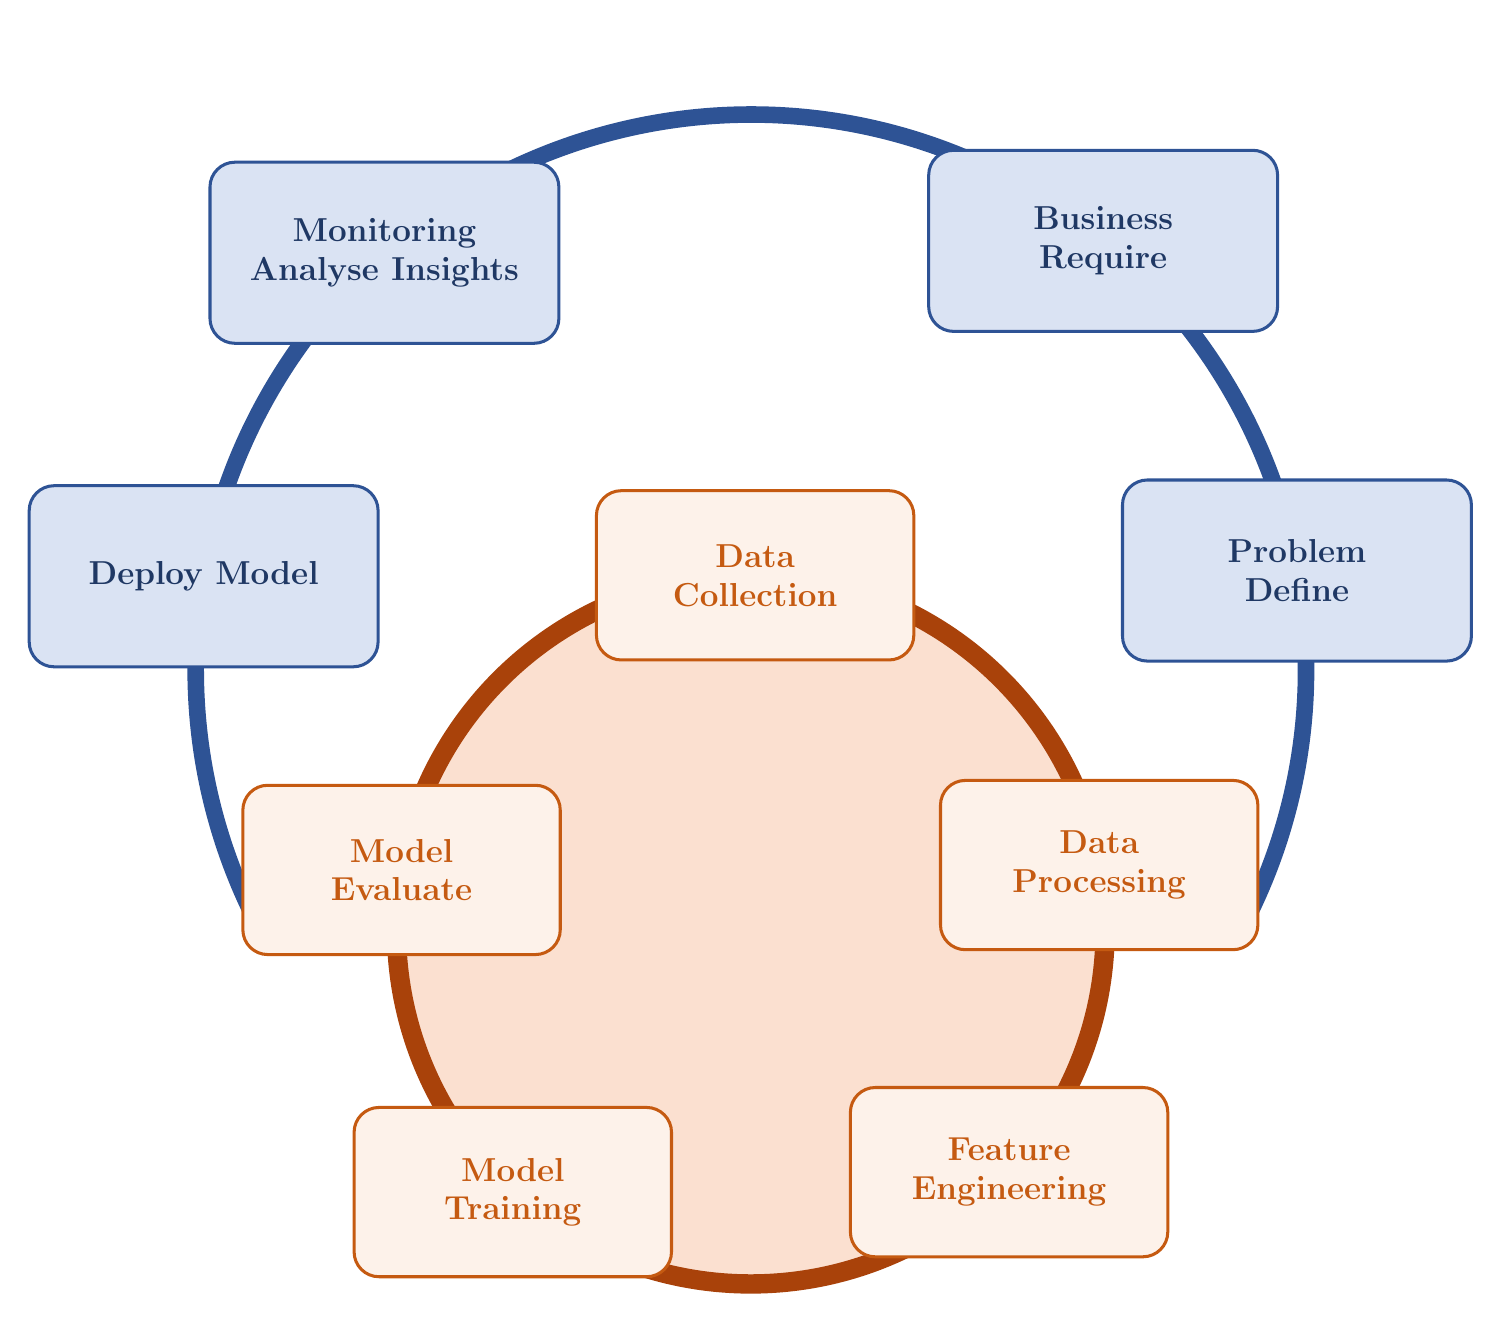
\begin{tikzpicture}[
  hopxanh/.style={
    draw=cXanhVien, line width=1.1pt, fill=cXanhNen, rounded corners=9pt,
    align=center, inner sep=4pt, text width=4.15cm, minimum height=2.3cm,
    font=\large\bfseries, text=cXanhChu
  },
  hopcam/.style={
    draw=cCamVien, line width=1.1pt, fill=cCamHop, rounded corners=9pt,
    align=center, inner sep=4pt, text width=3.75cm, minimum height=2.15cm,
    font=\large\bfseries, text=cCamVien
  }
]

% ── Hai duong tron: tam va ban kinh do tu ban goc ──
% Duong tron xanh : tam (0; 3,30) ban kinh 7,05 cm - chi ve cung tu -12 den 194 do
% Duong tron cam  : tam (0; 0)    ban kinh 4,50 cm - ve tron va to mau
\def\Rx{7.05}   \def\Cy{3.30}
\def\Rc{4.50}

% Dia tron cam ve TRUOC de cung xanh khong bi che
\fill[cCamNen] (0,0) circle (\Rc);
\draw[cCamVong, line width=7pt] (0,0) circle (\Rc);

% Cung tron xanh o ngoai. Hai dau keo den -27 va 207 do de diem cuoi nam HAN vao trong
% hop 'Xu ly du lieu' va 'Danh gia mo hinh'; hop ve sau nen che kin dau cung, nhin ra hai
% vong noi lien nhau dung nhu ban goc. De -12/194 do thi dau cung ho ra ngoai mep hop,
% thanh ra hai net xanh bi cut lung lo.
\draw[cXanhVien, line width=6pt]
  ([shift={(0,\Cy)}]-27:\Rx) arc[start angle=-27, end angle=207, radius=\Rx];

% ── Bon hop tren cung xanh ──
\node[hopxanh] at ($(0,\Cy)+(131.3:\Rx)$) {\Lmonitor};
\node[hopxanh] at ($(0,\Cy)+( 50.6:\Rx)$) {\Lbusiness};
\node[hopxanh] at ($(0,\Cy)+( 10.3:\Rx)$) {\Lproblem};
\node[hopxanh] at ($(0,\Cy)+(170.3:\Rx)$) {\Ldeploy};

% ── Nam hop tren vong cam ──
\node[hopcam] at ( 89.3:\Rc) {\Lcollect};
\node[hopcam] at ( 10.5:\Rc) {\Lprocess};
\node[hopcam] at (-43.2:\Rc) {\Lfeature};
\node[hopcam] at (227.8:\Rc) {\Ltrain};
\node[hopcam] at (170.3:\Rc) {\Levaluate};

\end{tikzpicture}
\end{document}
"
%
%  GHI CHU: ban goc viet sai chinh ta "Model Traing". Ban ve lai dung
%  "Model Training". Muon giu nguyen loi cua ban goc thi sua lai o \Ltrain.
% =============================================================================
\documentclass[12pt]{article}
\usepackage{fontspec}
\setmainfont{TeX Gyre Termes}          % chu co chan, khop kieu chu ban goc
% Khung giay do vua voi so do: TikZ do duoc 522,2 x 447,7 pt = 18,4 x 15,8 cm,
% cong dong tieu de va le nen cao 18,5 cm thi hinh nam gon 1 trang, khong bi day sang trang 2.
\usepackage[margin=0.5cm,paperwidth=19.5cm,paperheight=18.5cm]{geometry}
\usepackage{tikz}
\usetikzlibrary{arrows.meta,calc}
\pagestyle{empty}

% ── Bang mau lay tu anh render cua slide goc ──
\definecolor{cXanhVien}{HTML}{2E5395}   % vien va cung tron xanh
\definecolor{cXanhNen}{HTML}{DAE3F3}    % nen hop xanh
\definecolor{cXanhChu}{HTML}{1F3864}    % chu trong hop xanh
\definecolor{cCamVien}{HTML}{C55A11}    % vien hop cam va chu cam
\definecolor{cCamVong}{HTML}{A9420A}    % vanh tron cam dam
\definecolor{cCamNen}{HTML}{FBE0D0}     % nen dia tron cam
\definecolor{cCamHop}{HTML}{FDF2EA}     % nen hop cam

% ── Nhan hai ngon ngu ──
\providecommand{\LANGVI}{0}
\ifnum\LANGVI=1
  \def\Ltieude{Vòng đời học máy}
  \def\Lmonitor{Giám sát\\Phân tích thông tin}
  \def\Lbusiness{Yêu cầu\\nghiệp vụ}
  \def\Lproblem{Xác định\\bài toán}
  \def\Ldeploy{Triển khai mô hình}
  \def\Lcollect{Thu thập\\dữ liệu}
  \def\Lprocess{Xử lý\\dữ liệu}
  \def\Lfeature{Sinh\\đặc trưng}
  \def\Ltrain{Huấn luyện\\mô hình}
  \def\Levaluate{Đánh giá\\mô hình}
\else
  \def\Ltieude{ML Life Cycle}
  \def\Lmonitor{Monitoring\\Analyse Insights}
  \def\Lbusiness{Business\\Require}
  \def\Lproblem{Problem\\Define}
  \def\Ldeploy{Deploy Model}
  \def\Lcollect{Data\\Collection}
  \def\Lprocess{Data\\Processing}
  \def\Lfeature{Feature\\Engineering}
  \def\Ltrain{Model\\Training}
  \def\Levaluate{Model\\Evaluate}
\fi

\begin{document}
\noindent{\Large\bfseries\color{cXanhChu}$\diamond$~\Ltieude}\par
\vspace{2mm}
\centering
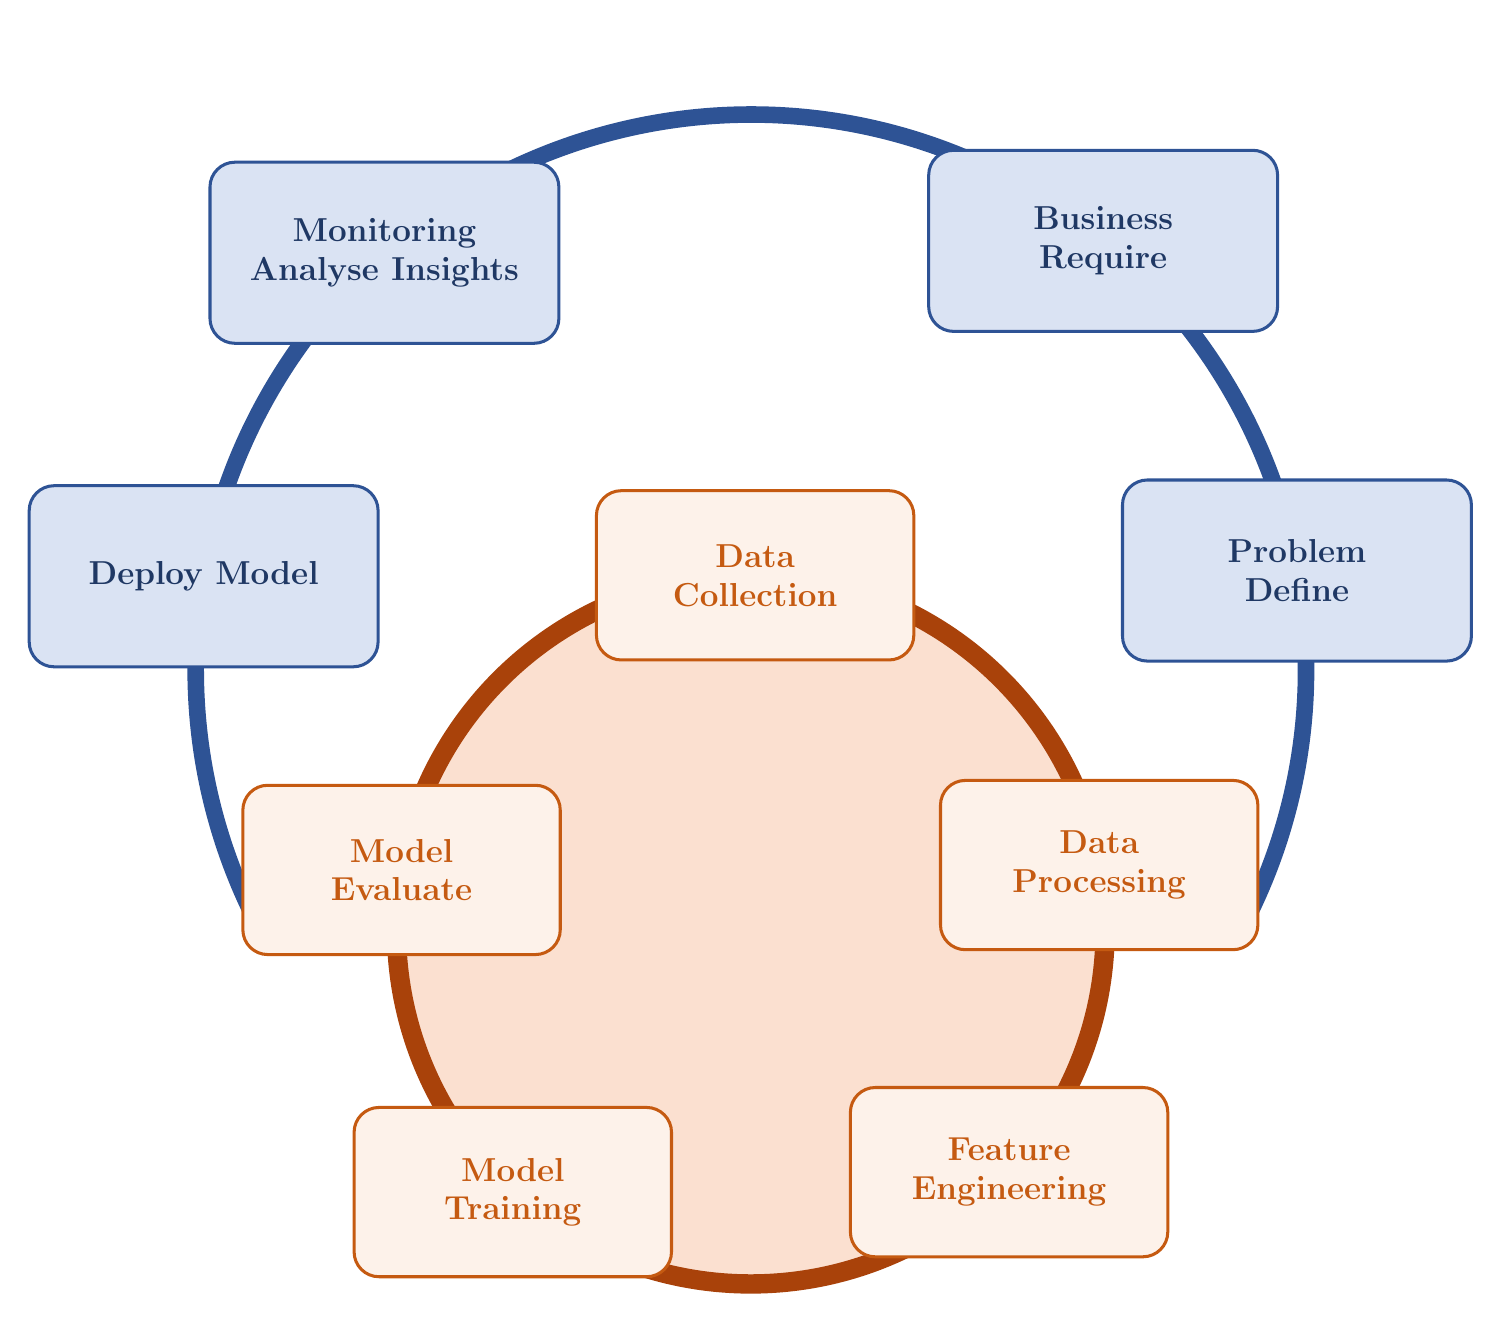
\begin{tikzpicture}[
  hopxanh/.style={
    draw=cXanhVien, line width=1.1pt, fill=cXanhNen, rounded corners=9pt,
    align=center, inner sep=4pt, text width=4.15cm, minimum height=2.3cm,
    font=\large\bfseries, text=cXanhChu
  },
  hopcam/.style={
    draw=cCamVien, line width=1.1pt, fill=cCamHop, rounded corners=9pt,
    align=center, inner sep=4pt, text width=3.75cm, minimum height=2.15cm,
    font=\large\bfseries, text=cCamVien
  }
]

% ── Hai duong tron: tam va ban kinh do tu ban goc ──
% Duong tron xanh : tam (0; 3,30) ban kinh 7,05 cm - chi ve cung tu -12 den 194 do
% Duong tron cam  : tam (0; 0)    ban kinh 4,50 cm - ve tron va to mau
\def\Rx{7.05}   \def\Cy{3.30}
\def\Rc{4.50}

% Dia tron cam ve TRUOC de cung xanh khong bi che
\fill[cCamNen] (0,0) circle (\Rc);
\draw[cCamVong, line width=7pt] (0,0) circle (\Rc);

% Cung tron xanh o ngoai. Hai dau keo den -27 va 207 do de diem cuoi nam HAN vao trong
% hop 'Xu ly du lieu' va 'Danh gia mo hinh'; hop ve sau nen che kin dau cung, nhin ra hai
% vong noi lien nhau dung nhu ban goc. De -12/194 do thi dau cung ho ra ngoai mep hop,
% thanh ra hai net xanh bi cut lung lo.
\draw[cXanhVien, line width=6pt]
  ([shift={(0,\Cy)}]-27:\Rx) arc[start angle=-27, end angle=207, radius=\Rx];

% ── Bon hop tren cung xanh ──
\node[hopxanh] at ($(0,\Cy)+(131.3:\Rx)$) {\Lmonitor};
\node[hopxanh] at ($(0,\Cy)+( 50.6:\Rx)$) {\Lbusiness};
\node[hopxanh] at ($(0,\Cy)+( 10.3:\Rx)$) {\Lproblem};
\node[hopxanh] at ($(0,\Cy)+(170.3:\Rx)$) {\Ldeploy};

% ── Nam hop tren vong cam ──
\node[hopcam] at ( 89.3:\Rc) {\Lcollect};
\node[hopcam] at ( 10.5:\Rc) {\Lprocess};
\node[hopcam] at (-43.2:\Rc) {\Lfeature};
\node[hopcam] at (227.8:\Rc) {\Ltrain};
\node[hopcam] at (170.3:\Rc) {\Levaluate};

\end{tikzpicture}
\end{document}
